% !TeX program = pdflatex
\documentclass[12pt]{article}

\usepackage{graphicx}
\usepackage{amsmath}
\usepackage{array}
\usepackage{fontspec}
\usepackage{amsfonts}
\usepackage{fancyhdr}
\usepackage{geometry}
\usepackage{subfigure}
\usepackage{caption}
\usepackage{karnaugh-map}
\usepackage{bm}
\usepackage[table]{xcolor}
\usepackage{float}
\usepackage{tikz}
\usepackage{hyperref}


\geometry{letterpaper, margin=1in}
\graphicspath{ {../images/} }

% Header and Footer
\pagestyle{fancy}
\fancyhf{}
\fancyhead[L]{CSE 2301 - Final Exam Study Guide}
\fancyhead[R]{\thepage}
\setlength{\headheight}{15pt}

\author{Arturo Salinas-Aguayo}
\title{Final Exam Study Guide}
% theorem set
\newtheorem{example}{Example}
% Example block environment
\newenvironment{examp}
{
    \vspace{0.5cm}
    \hrule
    \begin{example}\upshape
}
{
    \end{example}
    \hrule
    \vspace{0.5cm}
}

\newcommand{\closure}[2][3]{%
	{}\mkern#1mu\overline{\mkern-#1mu#2}}
\newcommand\ncoverline[1]{\mkern1mu\overline{\mkern-1mu#1\mkern-1mu}\mkern1mu}

\begin{document}

% Title Page
\begin{titlepage}
	\centering
	\vspace*{3cm}
	\huge\textbf{Final Exam Study Guide}\\
	\vspace{5cm}
	\Large\textbf{Arturo Salinas-Aguayo}\\
	\normalsize
	CSE 2301: Principles and Practice of Digital Logic Design\\
	Dr. Mohammad Khan, Section 003L-1248\\
	Electrical and Computer Engineering Department
	\vfill
	
\includegraphics[scale=0.1]{uconnlogo}\\
	College of Engineering, University of Connecticut\\
	\scriptsize{Coded in \LaTeX}
	\vspace*{1cm}
\end{titlepage}
\tableofcontents
\newpage
\section{Exam 1: From the Top}
\subsection{Topical Guide Objectives}
\begin{enumerate}
	\item Use Vocabulary such as:
	      \begin{itemize}
		      \item Ohm's Law: $V = IR$
		      \item Kirchoff's Current Law: $\sum I_{in} = \sum I_{out}$
		      \item Kirchoff's Voltage Law: $\sum V_{in} = \sum V_{out}$
		      \item TTL: Transistor-Transistor Logic (Low 0V-2V, High 2-5V)
		      \item CMOS: Complementary Metal-Oxide-Semiconductor (Low 0-1.5V, High 3.5-5V)
		      \item VLSI: Very Large Scale Integration (Typically 100,000+
		            transistors)
		      \item LSI: Large Scale Integration (Typically 1,000-100,000
		            transistors)
		      \item MSI: Medium Scale Integration (Typically 100-1000
		            transistors)
		      \item SSI: Small Scale Integration (Typically 10-100 transistors)
		      \item Radix: Base of a number system
		      \item Radix Economy: The number of bits required to represent a number
		      \item Essential Prime Implicant: A prime implicant that covers a
		            minterm not covered by any other prime implicant
		      \item Secondary Prime Implicant: A prime implicant that covers a
		            minterm already covered by another prime implicant
	      \end{itemize}
	\item Be able to convert between different Number Systems including
	      Decimal, Binary, Octal, Hexadecimal, 1's and 2's Complement.
	\item Understand how XS3 (Excess-3), BCD, and Gray code encoding work.
	\item Be able to perform basic arithmetic on above number systems.
	\item Be able to reduce Boolean Logic algebraically
	\item Be able to use DeMorgan's Theorem to simplify Boolean Logic and switch
	      to pure NAND or NOR gate implementations.
	\item Be able to set up and solve Karnaugh Maps up to 5 variables
\end{enumerate}

\subsection{Number Systems and Conversion}
\subsubsection{Basic Binary Arithmetic}
This is very similar to standard math in decimal, except that
you only have two digits to work with, 0 and 1. The rules are
the same, but the carry is a bit different. For example:
\begin{examp}
	\[
		\begin{array}{r}
			1101  \\
			+1011 \\
			\hline
			11000
		\end{array}
	\]
\end{examp}

\textbf{Overflow} - Occurs when adding two positive numbers produces
a negative answer or if adding two negative numbers gives a positive
answer.

In 2's Compliment, an overflow occurs if an donly if the carry out
of the sign position is not equal to the carry into the sign position.


\subsubsection{Decimal to Binary:}
\begin{examp}
	Given:
	\[
		37_{10}\\
	\]
	Convert to Binary Sign Magnitude and 2's Compliment in 8-bit
	binary.

	\textit{Recall:} Sign Magnitude simply utilizes the MSB (Big Endian)
	to denote the sign of the number.

	Start by appending the MSB with the sign bit. 0 is positive, 1
	is negative.
	\[
		0XXXXXXXX
	\]

	\begin{align*}
		2  / 37 \quad &                     \\
		2  / 18 \quad & \text{Remainder: 1} \\
		2  / 9 \quad  & \text{Remainder: 0} \\
		2  / 4 \quad  & \text{Remainder: 1} \\
		2  / 2 \quad  & \text{Remainder: 0} \\
		2  / 1\quad   & \text{Remainder: 0} \\
		0\quad        & \text{Remainder: 1}
	\end{align*}
	This results in the following binary number recall start from the
	bottom and work your way up when working with whole numbers (ie
	not decimal values).
	\[
		100101_2
	\]
	But this is still not finished, the question asks for 8 bits,
	the arithmetic produced 6 bits, and we already have our MSB from
	the signed operation, so we fill in one more bit via
	\textit{sign extension}. Propogate the sign bit until you reach
	the desired bits.
	\[
		00100101_2
	\]
	For the 2's Compliment, we start at our six bit result from above.
	You flip the bits, that is, 1 becomes 0, and 0 becomes 1, why?
	Because... that's how you do it.
	\[
		011010_2
	\]
	Add $1_2$
	\[
		011011_2
	\]
	Extend the sign.
	\[
		00011011_2
	\]
\end{examp}

\begin{examp}
	Let's move quicker now. \newline
	Given:
	\[
		-12_{10}
	\]
	Negative, fill in MSB.
	\[
		1XXXXXXX
	\]
	\begin{align*}
		2 / 12 &                             \\
		2 / 6  & \quad & \text{Remainder: 0} \\
		2 / 3  & \quad & \text{Remainder: 0} \\
		2 / 1  & \quad & \text{Remainder: 1} \\
		0      & \quad & \text{Remainder: 1} \\
	\end{align*}
	Signed Magnitude with sign extension:
	\[
		11111100_2
	\]
	2's Compliment:
	\[
		11110100_2
	\]
	Take a moment to convince yourself you can do this.
\end{examp}
\subsubsection{Decimal Conversion and IEEE 754}
\begin{examp}
	Decimal Conversion \newline
	Given:
	\[
		-0.625_{10}
	\]
	Convert to Binary.

	Instead of dividing until we reach 0, we multiply by the
	Radix until we no longer conatin a decimal number to
	multiply.

	\begin{align*}
		0.625 \times 2 & = 1.250 \quad \text{Remainder: 1} \\
		0.250 \times 2 & = 0.500 \quad \text{Remainder: 0} \\
		0.500 \times 2 & = 1.000 \quad \text{Remainder: 1}
	\end{align*}

	This gets filled in the opposite direction. The first
	operation is our MSB now instead of the LSB as with whole
	numbers.
	\[
		.625_{10} = .101_2
	\]
\end{examp}
\begin{examp}
	Let's now extend this and convert this number to the IEEE
	754 32-bit single precision format standard.

	\textit{Recall:}
	\begin{itemize}
		\item Sign Bit - The first bit. A simple 0 or 1 as explained in Example 1
		\item Exponent - The next 8 bits represent the exponent in a biased form. A bias is added to the actual exponent to ensure that both positive and negative exponents can be represented as unsigned binary numbers. For single-precision, the bias is 127. This means:
		      \[
			      \text{Stored Exponent}  =\text{Actual Exponent}+127 \\
		      \]
		      For example, an actual exponent of 3 would be stored as \(3 + 127 = 130\) in binary. Similarly, an actual exponent of \(-2\) would be stored as \(-2 + 127 = 125\).
		\item Mantissa - The final 23 bits hold the \textit{mantissa}, which represents the significant digits of the number in binary. In scientific notation, the mantissa is the number we multiply by a power of 10 (or, in binary, a power of 2). For instance, in the decimal number $4.2 \times 10^1$, the mantissa is $4.2$, and the exponent is $1$.
	\end{itemize}
	The first bit is the sign bit, the next sector is  8 bits of exponent,
	followed by the final 23 bits of \textit{mantissa.} This is a simple
	concept, the mantissa is just what is normally the number we multiply
	by in scientific notation. (e.g $4.2E1$, 4.2 is the mantissa, 1 is the exponent)
	\begin{enumerate}
		\item Look at the sign and fill the MSB:
		      \[
			      .625_{10} \quad\text{Positive, MSB} \implies 0
		      \]
		\item Convert to binary if necessary and adjust to scientific notation.
		      \[
			      .625_{10} =  .101_2 = 1.01 \times 2^{-1}
		      \]
		\item Hopefully this is becoming clearer now.

		      Our Mantissa, or our \textit{Fraction} is \(1.01\)\newline
		      Our exponent is \(-1\)
		\item Let's focus on the Fraction first.
		      The leading \(1\) in \(1.01 \times 2^{-1}\) is ignored. We only
		      care about the \(.01\).

		      The fraction portion of the standard is 23 bits long for a single
		      precision number. So our last 23 bits are:
		      \[
			      010 0000 0000 0000 0000 0000
		      \]
		\item Now we add the Bias to the exponent and convert that to binary.
		      \[
			      -1 + 127 = 126
		      \]
		      \textit{Quick Maffs:}
		      Engrain \(2^7 = 128\) into your head.
		      \[
			      \implies 1111111_2 = 127_{10}
		      \]
		      \[
			      \implies 1111110_2 = 126_{10}
		      \]
		      Remember that the exponent is 8 bits, so add the leading 0.
		      \[
			      01111110_2
		      \]
		\item That leaves the final number:
		      \[
			      0 01111110 010 0000 0000 0000 0000 0000_2
		      \]
	\end{enumerate}

\end{examp}
\subsubsection{Radix and Other Systems}
The Radix is the base of a number system. The Radix Economy is the number of
bits required to represent a number. It can be calculated by:
\[
	\text{Radix Economy} = \log_2(\text{Radix})]
\]
The higher the number, the more efficient the system is. The peak efficiency is
somewhere around \(e = 2.718\).
To calculate the radix economy of a given number, you multiply the amount
of digits by the base.
\begin{examp}
	\[
		111_{10} \implies 3 \times 10 = 30\\
		1101111_2 \implies 7 \times 2 = 14\\
		157_8 \implies 3 \times 8 = 24\\
	\]
\end{examp}

The most common Radices are:
\begin{itemize}
	\item Decimal - Base 10\\
	\item Binary - Base 2\\
	\item Octal - Base 8\\
	\item Hexadecimal - Base 16
\end{itemize}
To convert between these systems, you can use the following:
\begin{examp}
	Convert the following numbers to the specified base.
	\begin{enumerate}
		\item \(101101_2 \rightarrow 8\)
		      Group the numbers in sets of 3. Start from the LSB.
		      101  101    that's 5 and 5. Therefore, 55 in Octal.
		      \begin{align*}
			      101101_2 & = 1 \times 2^5 + 0 \times 2^4 + 1 \times 2^3 + 1 \times 2^2 + 0 \times 2^1 + 1 \times 2^0 \\
			               & = 32 + 0 + 8 + 4 + 0 + 1 = 45_{10}
		      \end{align*}
		      Now convert to Octal.
		      \begin{align*}
			      45_{10} & = 5 \times 8^1 + 5 \times 8^0 \\
			              & = 55_8
		      \end{align*}
		\item \(101101_2 \rightarrow 16\)
		      Group the numbers in sets of 4. Start from the LSB.
		      Now convert to Hexadecimal.
		      \[
			      45_{10}  = 2D_{16}
		      \]
	\end{enumerate}
\end{examp}
\subsubsection{XS3, BCD, and Gray Code}
These are different binary codes which are used for different purposes.
\begin{itemize}
	\item BCD is simply the binary representation of a decimal number. With each
	      digit represented by 4 bits. This is useful for arithmetic operations.
	\item XS3 is a
	      conversion that adds 3. This means that we will have don't care's for the
	      values of 6, 7, 8, and 9.
	\item Gray code is a binary code where only one bit
	      changes at a time. This is useful for error detection and correction.
\end{itemize}
\begin{examp}
	Convert the following numbers to the specified code.
	\begin{enumerate}
		\item \(101101_2 \rightarrow XS3\)\\
		      Just add 3 to the number.
		      \begin{align*}
			      101101_2 & = 110110_2
		      \end{align*}
		\item \(101101_2 \rightarrow BCD\)\\
		      This is a bit more involved. We need to convert the number to decimal first.
		      \[64 + 16 + 8 + 1 = 89_{10}\]
		      8 is 1000 in binary, 9 is 1001 in binary.
		      so, 89 in BCD is 1000 1001
		\item \(101101_2 \rightarrow Gray\)
		      \begin{align*}
			      101101_2 & = 111111_2
		      \end{align*}
	\end{enumerate}
\end{examp}
\subsection{Boolean Algebra}
\subsubsection{Basic Laws}
\begin{itemize}
	\item \textbf{Commutative Law:} \(A + B = B + A\), \(AB = BA\)\\
	      We can flip the order of the operands.
	\item \textbf{Associative Law:} \(A + (B + C) = (A + B) + C\), \(A(BC) = (AB)C\)\\
	      We can change the grouping of the operands.
	\item \textbf{Distributive Law:} \(A(B + C) = AB + AC\), \(A + BC = (A + B)(A + C)\)\\
	      We can distribute the operation across the operands.
	\item \textbf{Identity Law:} \(A + 0 = A\), \(A \cdot 1 = A\)\\
	      We can \textbf{add} 0 or \textbf{multiply} by 1 without changing the value.
	\item \textbf{Complement Law:} \(A + \closure{A} = 1\), \(A \cdot \closure{A} = 0\)\\
	      The or of a variable and its complement is always 1, the and of a variable and its complement is always 0.
	\item \textbf{Involution Law:} \(\closure{\closure{A}} = A\)\\
	      The compliment of the compliment is the original variable.
	\item \textbf{Absorption Law:} \(A + AB = A\), \(A(A + B) = A\)
	\item \textbf{DeMorgan's Theorem:} \(\closure{A + B} = \closure{A} \cdot \closure{B}\), \(\closure{A \cdot B} = \closure{A} + \closure{B}\)
\end{itemize}
\subsubsection{Conversion Using DeMorgan's Theorem}
The conversion process takes a bit getting used to, however it is straight forward.
\begin{enumerate}
	\item Start with the original expression.
	\item Apply DeMorgan's Theorem.
	\item Simplify the expression.
	\item Apply DeMorgan's Theorem again.
	\item Simplify the expression.
	\item If necessary, apply DeMorgan's Theorem again.
\end{enumerate}
\begin{examp}
	Utilize DeMorgan's Theorem to implement the following logic using 2-input
	or 3-input NAND gates only:
	\[
		F = \closure{A}(B+C) + CD
	\]
	First, expand the expression.
	\[
		F = \closure{A}B + \closure{A}C + CD
	\]
	Now, start by adding two bars to the entire expression.
	\[
		F = \closure{\closure{\closure{A}B + \closure{A}C + CD}}
	\]
	Bring down the outermost bar and exchange our \(+\) for a \(\cdot\).
	\[
		F = \closure{\closure{A}B \cdot \closure{\closure{A}C} \cdot \closure{CD}}
	\]
	Daas it.
	\begin{figure}[H]
		\resizebox{15cm}{!}{
			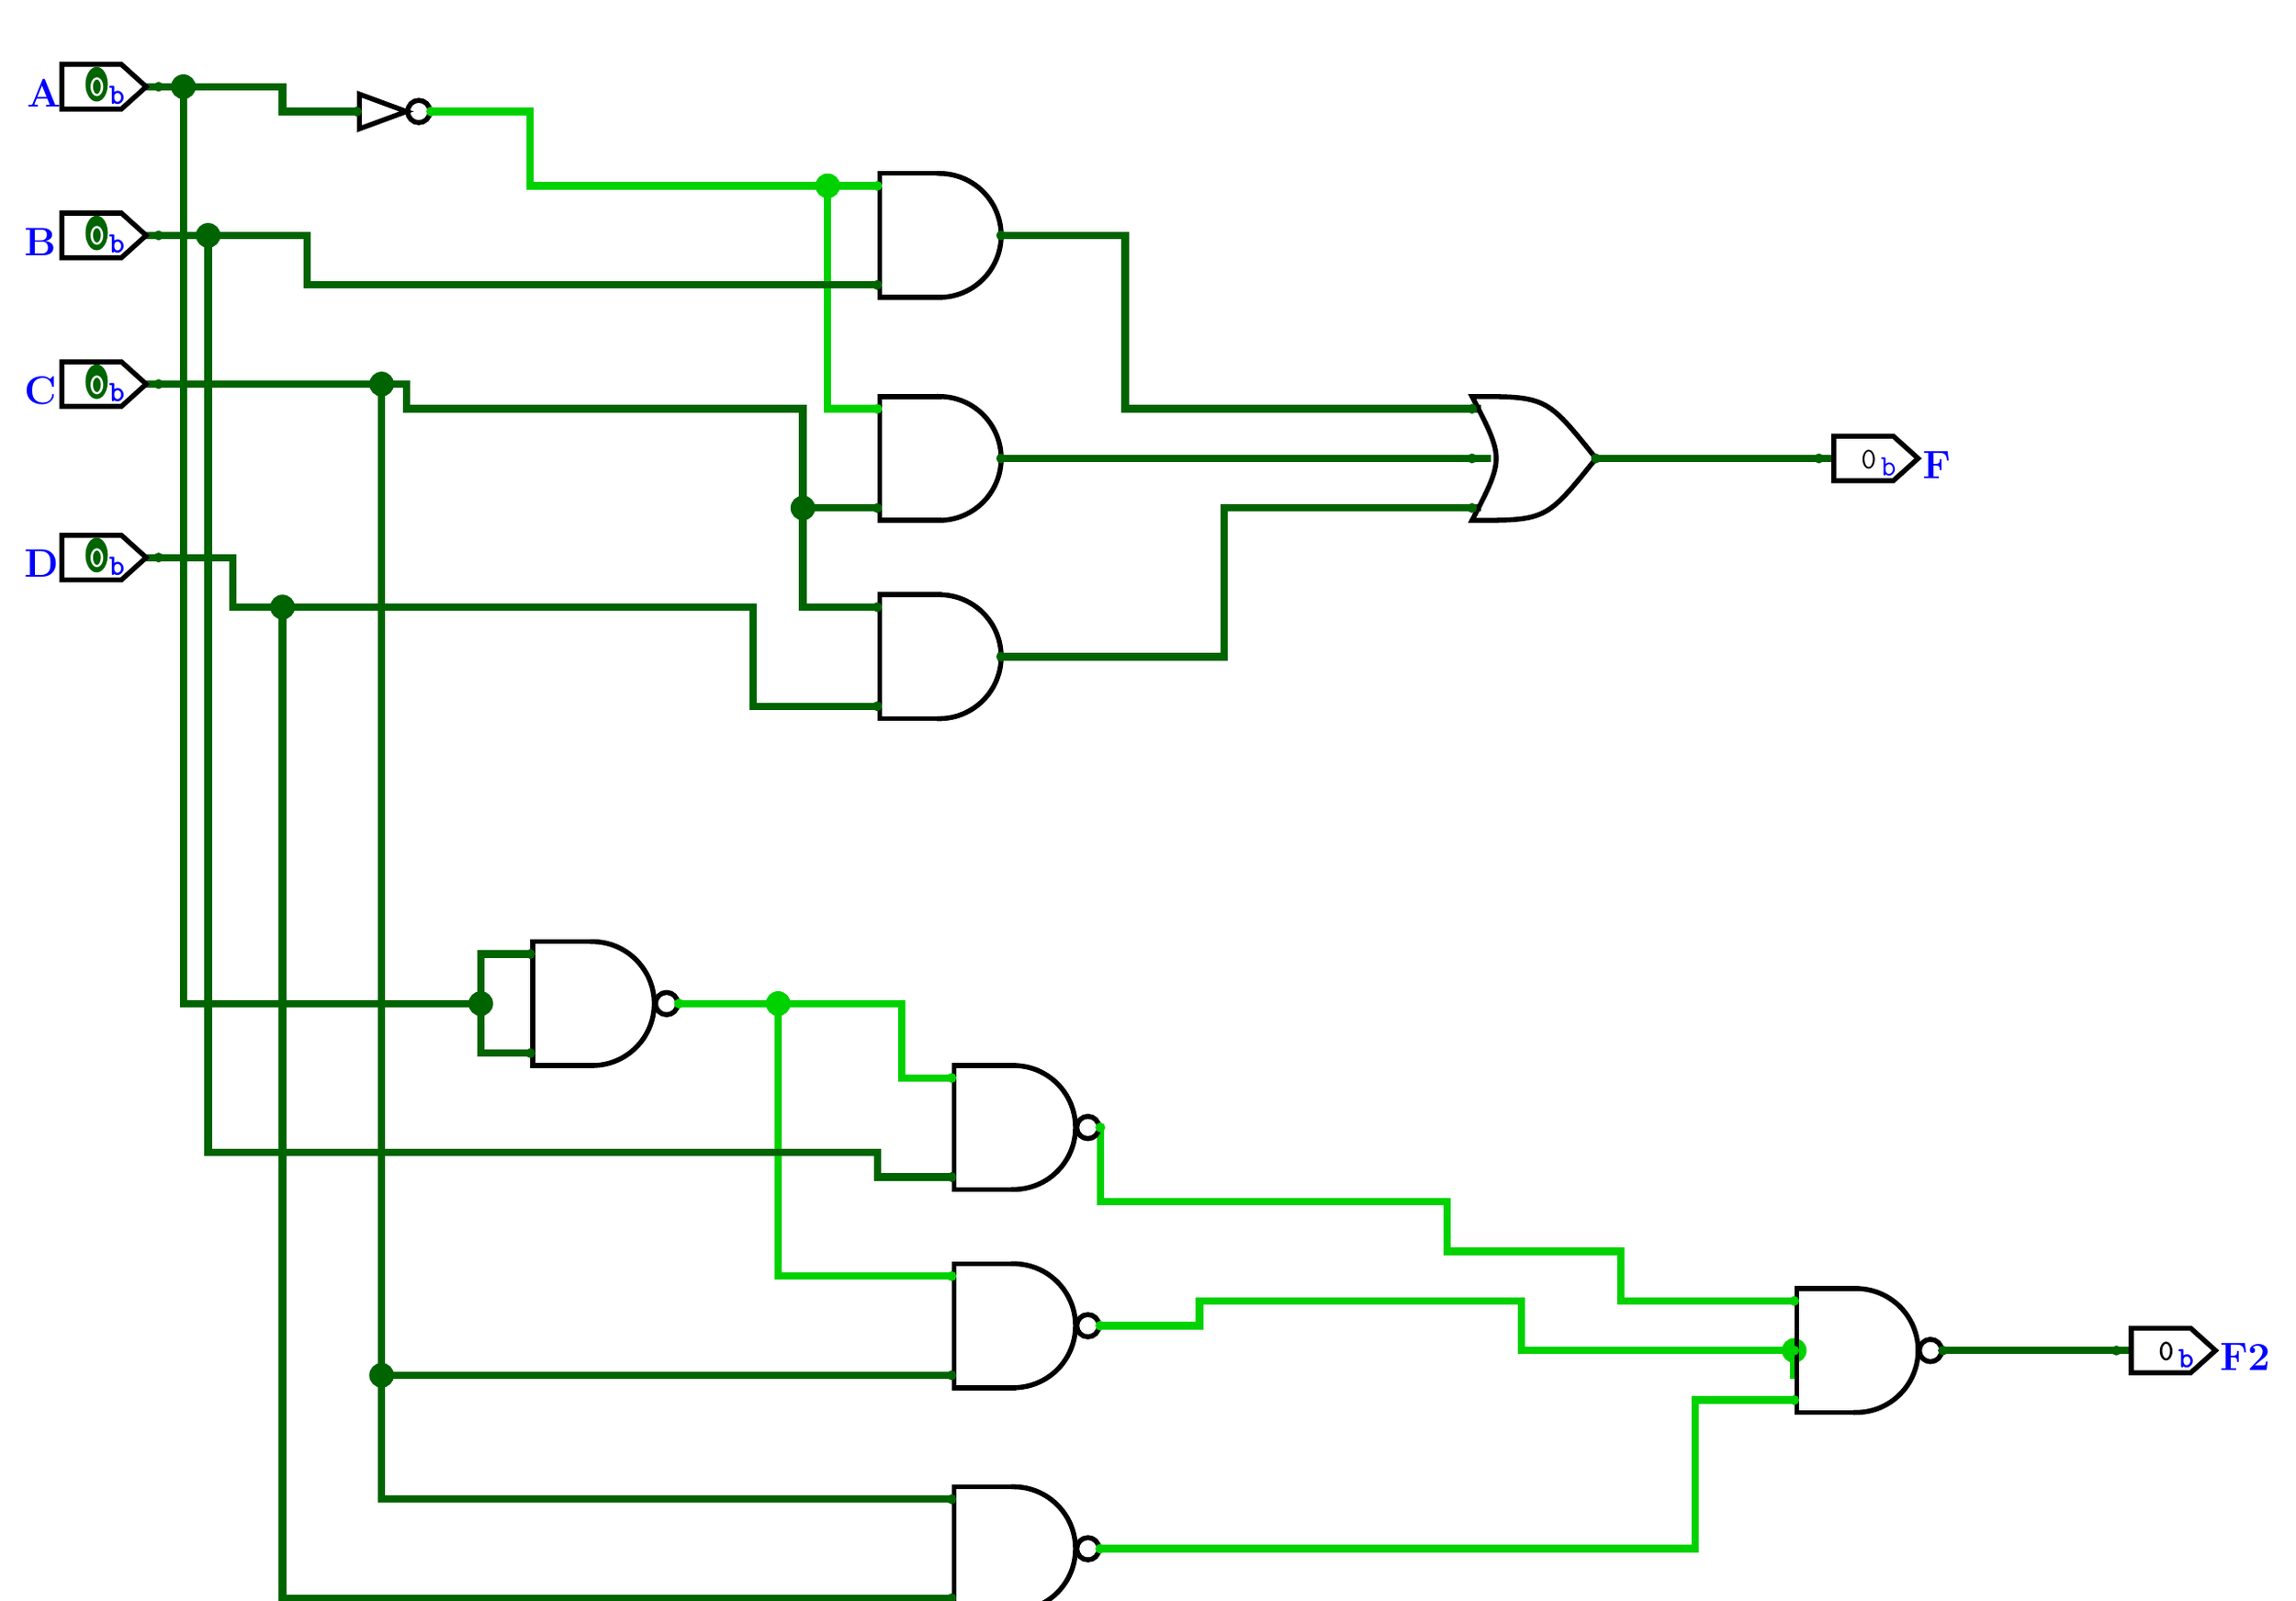
\begin{tikzpicture}[x=1pt,y=-1pt,line cap=rect]
				\def\logisimfontA#1{\fontfamily{lmr}\selectfont#1} % Use Latin Modern Roman
				\def\logisimfontB#1{\fontfamily{lmtt}\selectfont#1} % Use Latin Modern Monospace
				\definecolor{custcol_0_0_ff}{RGB}{0, 0, 255}
				\definecolor{custcol_0_64_0}{RGB}{0, 100, 0}
				\definecolor{custcol_0_0_0}{RGB}{0, 0, 0}
				\definecolor{custcol_0_d2_0}{RGB}{0, 210, 0}
				\definecolor{custcol_ff_ff_ff}{RGB}{255, 255, 255}
				\draw [line width=3.0pt, custcol_0_64_0 ]  (639.0,165.0) -- (729.0,165.0) ;
				\draw [line width=3.0pt, custcol_0_64_0 ]  (779.0,525.0) -- (849.0,525.0) ;
				\draw [line width=3.0pt, custcol_0_d2_0 ]  (169.0,25.0) -- (209.0,25.0) -- (209.0,55.0) -- (329.0,55.0) ;
				\draw [line width=3.0pt, custcol_0_d2_0 ]  (349.0,55.0) -- (329.0,55.0) -- (329.0,145.0) -- (349.0,145.0) ;
				\draw [line width=3.0pt, custcol_0_d2_0 ]  (269.0,385.0) -- (309.0,385.0) -- (359.0,385.0) -- (359.0,415.0) -- (379.0,415.0) ;
				\draw [line width=3.0pt, custcol_0_d2_0 ]  (309.0,385.0) -- (309.0,495.0) -- (379.0,495.0) ;
				\draw [line width=3.0pt, custcol_0_64_0 ]  (379.0,625.0) -- (109.0,625.0) -- (109.0,225.0) -- (299.0,225.0) -- (299.0,265.0) -- (349.0,265.0) ;
				\draw [line width=3.0pt, custcol_0_64_0 ]  (319.0,185.0) -- (319.0,225.0) -- (349.0,225.0) ;
				\draw [line width=3.0pt, custcol_0_64_0 ]  (189.0,385.0) -- (189.0,365.0) -- (209.0,365.0) ;
				\draw [line width=3.0pt, custcol_0_64_0 ]  (139.0,25.0) -- (109.0,25.0) -- (109.0,15.0) -- (69.0,15.0) -- (69.0,385.0) -- (189.0,385.0) -- (189.0,405.0) -- (209.0,405.0) ;
				\draw [line width=3.0pt, custcol_0_d2_0 ]  (439.0,435.0) -- (439.0,465.0) -- (579.0,465.0) -- (579.0,485.0) -- (649.0,485.0) -- (649.0,505.0) -- (719.0,505.0) ;
				\draw [line width=3.0pt, custcol_0_64_0 ]  (149.0,535.0) -- (149.0,585.0) -- (379.0,585.0) ;
				\draw [line width=3.0pt, custcol_0_64_0 ]  (79.0,75.0) -- (79.0,445.0) -- (349.0,445.0) -- (349.0,455.0) -- (379.0,455.0) ;
				\draw [line width=3.0pt, custcol_0_64_0 ]  (149.0,135.0) -- (159.0,135.0) -- (159.0,145.0) -- (319.0,145.0) -- (319.0,185.0) -- (349.0,185.0) ;
				\draw [line width=3.0pt, custcol_0_d2_0 ]  (439.0,515.0) -- (479.0,515.0) -- (479.0,505.0) -- (609.0,505.0) -- (609.0,525.0) -- (719.0,525.0) -- (719.0,535.0) ;
				\draw [line width=3.0pt, custcol_0_d2_0 ]  (719.0,545.0) -- (679.0,545.0) -- (679.0,605.0) -- (439.0,605.0) ;
				\fill [line width=3.0pt, custcol_0_64_0]  (79.0,75.0) ellipse (5.0 and 5.0 );
				\fill [line width=3.0pt, custcol_0_d2_0]  (309.0,385.0) ellipse (5.0 and 5.0 );
				\fill [line width=3.0pt, custcol_0_d2_0]  (329.0,55.0) ellipse (5.0 and 5.0 );
				\fill [line width=3.0pt, custcol_0_64_0]  (109.0,225.0) ellipse (5.0 and 5.0 );
				\fill [line width=3.0pt, custcol_0_d2_0]  (719.0,525.0) ellipse (5.0 and 5.0 );
				\fill [line width=3.0pt, custcol_0_64_0]  (149.0,535.0) ellipse (5.0 and 5.0 );
				\fill [line width=3.0pt, custcol_0_64_0]  (319.0,185.0) ellipse (5.0 and 5.0 );
				\fill [line width=3.0pt, custcol_0_64_0]  (189.0,385.0) ellipse (5.0 and 5.0 );
				\fill [line width=3.0pt, custcol_0_64_0]  (69.0,15.0) ellipse (5.0 and 5.0 );
				\fill [line width=3.0pt, custcol_0_64_0]  (149.0,135.0) ellipse (5.0 and 5.0 );
				\draw [line width=2.0pt, custcol_0_0_0 ]  (159.0,25.0) -- (140.0,18.0) -- (140.0,32.0) -- cycle;
				\draw [line width=2.0pt, custcol_0_0_0]  (164.0,25.0) ellipse (4.5 and 4.5 );
				\fill [line width=2.0pt, custcol_0_d2_0]  (169.0,25.0) ellipse (2.0 and 2.0 );
				\fill [line width=2.0pt, custcol_0_64_0]  (139.0,25.0) ellipse (2.0 and 2.0 );
				\draw [line width=2.0pt, custcol_0_0_0] (234.0,410.0) arc (90.0:-90.0:25.0 and 25.0 );
				\draw [line width=2.0pt, custcol_0_0_0 ]  (234.0,360.0) -- (210.0,360.0) -- (210.0,410.0) -- (234.0,410.0) ;
				\draw [line width=2.0pt, custcol_0_0_0]  (264.0,385.0) ellipse (4.5 and 4.5 );
				\fill [line width=2.0pt, custcol_0_d2_0]  (269.0,385.0) ellipse (2.0 and 2.0 );
				\fill [line width=2.0pt, custcol_0_64_0]  (209.0,365.0) ellipse (2.0 and 2.0 );
				\fill [line width=2.0pt, custcol_0_64_0]  (209.0,405.0) ellipse (2.0 and 2.0 );
				\draw [line width=2.0pt, custcol_0_0_0] (404.0,540.0) arc (90.0:-90.0:25.0 and 25.0 );
				\draw [line width=2.0pt, custcol_0_0_0 ]  (404.0,490.0) -- (380.0,490.0) -- (380.0,540.0) -- (404.0,540.0) ;
				\draw [line width=2.0pt, custcol_0_0_0]  (434.0,515.0) ellipse (4.5 and 4.5 );
				\fill [line width=2.0pt, custcol_0_d2_0]  (439.0,515.0) ellipse (2.0 and 2.0 );
				\fill [line width=2.0pt, custcol_0_d2_0]  (379.0,495.0) ellipse (2.0 and 2.0 );
				\fill [line width=2.0pt, custcol_0_64_0]  (379.0,535.0) ellipse (2.0 and 2.0 );
				\draw [line width=2.0pt, custcol_0_0_0] (404.0,630.0) arc (90.0:-90.0:25.0 and 25.0 );
				\draw [line width=2.0pt, custcol_0_0_0 ]  (404.0,580.0) -- (380.0,580.0) -- (380.0,630.0) -- (404.0,630.0) ;
				\draw [line width=2.0pt, custcol_0_0_0]  (434.0,605.0) ellipse (4.5 and 4.5 );
				\fill [line width=2.0pt, custcol_0_d2_0]  (439.0,605.0) ellipse (2.0 and 2.0 );
				\fill [line width=2.0pt, custcol_0_64_0]  (379.0,585.0) ellipse (2.0 and 2.0 );
				\fill [line width=2.0pt, custcol_0_64_0]  (379.0,625.0) ellipse (2.0 and 2.0 );
				\draw [line width=2.0pt, custcol_0_0_0] (744.0,550.0) arc (90.0:-90.0:25.0 and 25.0 );
				\draw [line width=2.0pt, custcol_0_0_0 ]  (744.0,500.0) -- (720.0,500.0) -- (720.0,550.0) -- (744.0,550.0) ;
				\draw [line width=2.0pt, custcol_0_0_0]  (774.0,525.0) ellipse (4.5 and 4.5 );
				\fill [line width=2.0pt, custcol_0_64_0]  (779.0,525.0) ellipse (2.0 and 2.0 );
				\fill [line width=2.0pt, custcol_0_d2_0]  (719.0,505.0) ellipse (2.0 and 2.0 );
				\fill [line width=2.0pt, custcol_0_d2_0]  (719.0,525.0) ellipse (2.0 and 2.0 );
				\fill [line width=2.0pt, custcol_0_d2_0]  (719.0,545.0) ellipse (2.0 and 2.0 );
				\draw [line width=2.0pt, custcol_0_0_0] (374.0,190.0) arc (90.0:-90.0:25.0 and 25.0 );
				\draw [line width=2.0pt, custcol_0_0_0 ]  (374.0,140.0) -- (350.0,140.0) -- (350.0,190.0) -- (374.0,190.0) ;
				\fill [line width=2.0pt, custcol_0_64_0]  (399.0,165.0) ellipse (2.0 and 2.0 );
				\fill [line width=2.0pt, custcol_0_d2_0]  (349.0,145.0) ellipse (2.0 and 2.0 );
				\fill [line width=2.0pt, custcol_0_64_0]  (349.0,185.0) ellipse (2.0 and 2.0 );
				\draw [line width=2.0pt, custcol_0_0_0] (374.0,270.0) arc (90.0:-90.0:25.0 and 25.0 );
				\draw [line width=2.0pt, custcol_0_0_0 ]  (374.0,220.0) -- (350.0,220.0) -- (350.0,270.0) -- (374.0,270.0) ;
				\fill [line width=2.0pt, custcol_0_64_0]  (399.0,245.0) ellipse (2.0 and 2.0 );
				\fill [line width=2.0pt, custcol_0_64_0]  (349.0,225.0) ellipse (2.0 and 2.0 );
				\fill [line width=2.0pt, custcol_0_64_0]  (349.0,265.0) ellipse (2.0 and 2.0 );
				\draw [line width=3.0pt, custcol_0_64_0 ]  (399.0,75.0) -- (449.0,75.0) -- (449.0,145.0) -- (589.0,145.0) -- (591.0,145.0) ;
				\draw [line width=3.0pt, custcol_0_64_0 ]  (399.0,165.0) -- (589.0,165.0) -- (595.0,165.0) ;
				\draw [line width=3.0pt, custcol_0_64_0 ]  (399.0,245.0) -- (489.0,245.0) -- (489.0,185.0) -- (589.0,185.0) -- (591.0,185.0) ;
				\draw [line width=2.0pt, custcol_0_0_0 ]  (639.0,165.0) .. controls  (619.0,140.0)  ..  (589.0,140.0) .. controls  (602.0,165.0)  ..  (589.0,190.0) .. controls  (619.0,190.0)  ..  (639.0,165.0) -- cycle ;
				\fill [line width=2.0pt, custcol_0_64_0]  (639.0,165.0) ellipse (2.0 and 2.0 );
				\fill [line width=2.0pt, custcol_0_64_0]  (589.0,145.0) ellipse (2.0 and 2.0 );
				\fill [line width=2.0pt, custcol_0_64_0]  (589.0,165.0) ellipse (2.0 and 2.0 );
				\fill [line width=2.0pt, custcol_0_64_0]  (589.0,185.0) ellipse (2.0 and 2.0 );
				\draw [line width=3.0pt, custcol_0_64_0 ]  (733.0,165.0) -- (730.0,165.0) ;
				\draw [line width=2.0pt, custcol_0_0_0 ]  (759.0,156.0) -- (769.0,165.0) -- (759.0,174.0) -- (735.0,174.0) -- (735.0,156.0) -- cycle;
				\logisimfontB{\fontsize{12pt}{12pt}\selectfont\node[inner sep=0, outer sep=0, custcol_0_0_ff, anchor=base west] at  (754.0,172.0)  {b};}
				\logisimfontB{\fontsize{12pt}{12pt}\selectfont\node[inner sep=0, outer sep=0, custcol_0_0_0, anchor=base west] at  (746.0,169.0)  {0};}
				\logisimfontA{\fontsize{16pt}{16pt}\fontseries{bx}\selectfont\node[inner sep=0, outer sep=0, custcol_0_0_ff, anchor=base west] at  (771.0,173.0)  {F};}
				\fill [line width=2.0pt, custcol_0_64_0]  (729.0,165.0) ellipse (2.0 and 2.0 );
				\draw [line width=3.0pt, custcol_0_64_0 ]  (853.0,525.0) -- (850.0,525.0) ;
				\draw [line width=2.0pt, custcol_0_0_0 ]  (879.0,516.0) -- (889.0,525.0) -- (879.0,534.0) -- (855.0,534.0) -- (855.0,516.0) -- cycle;
				\logisimfontB{\fontsize{12pt}{12pt}\selectfont\node[inner sep=0, outer sep=0, custcol_0_0_ff, anchor=base west] at  (874.0,532.0)  {b};}
				\logisimfontB{\fontsize{12pt}{12pt}\selectfont\node[inner sep=0, outer sep=0, custcol_0_0_0, anchor=base west] at  (866.0,529.0)  {0};}
				\logisimfontA{\fontsize{16pt}{16pt}\fontseries{bx}\selectfont\node[inner sep=0, outer sep=0, custcol_0_0_ff, anchor=base west] at  (891.0,533.0)  {F2};}
				\fill [line width=2.0pt, custcol_0_64_0]  (849.0,525.0) ellipse (2.0 and 2.0 );
				\draw [line width=2.0pt, custcol_0_0_0] (374.0,100.0) arc (90.0:-90.0:25.0 and 25.0 );
				\draw [line width=2.0pt, custcol_0_0_0 ]  (374.0,50.0) -- (350.0,50.0) -- (350.0,100.0) -- (374.0,100.0) ;
				\fill [line width=2.0pt, custcol_0_64_0]  (399.0,75.0) ellipse (2.0 and 2.0 );
				\fill [line width=2.0pt, custcol_0_d2_0]  (349.0,55.0) ellipse (2.0 and 2.0 );
				\fill [line width=2.0pt, custcol_0_64_0]  (349.0,95.0) ellipse (2.0 and 2.0 );
				\draw [line width=2.0pt, custcol_0_0_0] (404.0,460.0) arc (90.0:-90.0:25.0 and 25.0 );
				\draw [line width=2.0pt, custcol_0_0_0 ]  (404.0,410.0) -- (380.0,410.0) -- (380.0,460.0) -- (404.0,460.0) ;
				\draw [line width=2.0pt, custcol_0_0_0]  (434.0,435.0) ellipse (4.5 and 4.5 );
				\fill [line width=2.0pt, custcol_0_d2_0]  (439.0,435.0) ellipse (2.0 and 2.0 );
				\fill [line width=2.0pt, custcol_0_d2_0]  (379.0,415.0) ellipse (2.0 and 2.0 );
				\fill [line width=2.0pt, custcol_0_64_0]  (379.0,455.0) ellipse (2.0 and 2.0 );
				\draw [line width=3.0pt, custcol_0_64_0 ]  (54.0,15.0) -- (59.0,15.0) -- (69.0,15.0) ;
				\draw [line width=2.0pt, custcol_0_0_0 ]  (44.0,24.0) -- (54.0,15.0) -- (44.0,6.0) -- (20.0,6.0) -- (20.0,24.0) -- cycle;
				\logisimfontB{\fontsize{12pt}{12pt}\selectfont\node[inner sep=0, outer sep=0, custcol_0_0_ff, anchor=base west] at  (39.0,22.0)  {b};}
				\fill [line width=2.0pt, custcol_0_64_0]  (34.0,14.0) ellipse (4.5 and 7.0 );
				\logisimfontB{\fontsize{12pt}{12pt}\selectfont\node[inner sep=0, outer sep=0, custcol_ff_ff_ff, anchor=base west] at  (31.0,19.0)  {0};}
				\logisimfontA{\fontsize{16pt}{16pt}\fontseries{bx}\selectfont\node[inner sep=0, outer sep=0, custcol_0_0_ff, anchor=base west] at  (6.0,23.0)  {A};}
				\fill [line width=2.0pt, custcol_0_64_0]  (59.0,15.0) ellipse (2.0 and 2.0 );
				\draw [line width=3.0pt, custcol_0_64_0 ]  (54.0,75.0) -- (59.0,75.0) -- (79.0,75.0) -- (119.0,75.0) -- (119.0,95.0) -- (349.0,95.0) ;
				\draw [line width=2.0pt, custcol_0_0_0 ]  (44.0,84.0) -- (54.0,75.0) -- (44.0,66.0) -- (20.0,66.0) -- (20.0,84.0) -- cycle;
				\logisimfontB{\fontsize{12pt}{12pt}\selectfont\node[inner sep=0, outer sep=0, custcol_0_0_ff, anchor=base west] at  (39.0,82.0)  {b};}
				\fill [line width=2.0pt, custcol_0_64_0]  (34.0,74.0) ellipse (4.5 and 7.0 );
				\logisimfontB{\fontsize{12pt}{12pt}\selectfont\node[inner sep=0, outer sep=0, custcol_ff_ff_ff, anchor=base west] at  (31.0,79.0)  {0};}
				\logisimfontA{\fontsize{16pt}{16pt}\fontseries{bx}\selectfont\node[inner sep=0, outer sep=0, custcol_0_0_ff, anchor=base west] at  (5.0,83.0)  {B};}
				\fill [line width=2.0pt, custcol_0_64_0]  (59.0,75.0) ellipse (2.0 and 2.0 );
				\draw [line width=3.0pt, custcol_0_64_0 ]  (54.0,135.0) -- (59.0,135.0) -- (149.0,135.0) -- (149.0,535.0) -- (379.0,535.0) ;
				\draw [line width=2.0pt, custcol_0_0_0 ]  (44.0,144.0) -- (54.0,135.0) -- (44.0,126.0) -- (20.0,126.0) -- (20.0,144.0) -- cycle;
				\logisimfontB{\fontsize{12pt}{12pt}\selectfont\node[inner sep=0, outer sep=0, custcol_0_0_ff, anchor=base west] at  (39.0,142.0)  {b};}
				\fill [line width=2.0pt, custcol_0_64_0]  (34.0,134.0) ellipse (4.5 and 7.0 );
				\logisimfontB{\fontsize{12pt}{12pt}\selectfont\node[inner sep=0, outer sep=0, custcol_ff_ff_ff, anchor=base west] at  (31.0,139.0)  {0};}
				\logisimfontA{\fontsize{16pt}{16pt}\fontseries{bx}\selectfont\node[inner sep=0, outer sep=0, custcol_0_0_ff, anchor=base west] at  (5.0,143.0)  {C};}
				\fill [line width=2.0pt, custcol_0_64_0]  (59.0,135.0) ellipse (2.0 and 2.0 );
				\draw [line width=3.0pt, custcol_0_64_0 ]  (54.0,205.0) -- (59.0,205.0) -- (89.0,205.0) -- (89.0,225.0) -- (109.0,225.0) ;
				\draw [line width=2.0pt, custcol_0_0_0 ]  (44.0,214.0) -- (54.0,205.0) -- (44.0,196.0) -- (20.0,196.0) -- (20.0,214.0) -- cycle;
				\logisimfontB{\fontsize{12pt}{12pt}\selectfont\node[inner sep=0, outer sep=0, custcol_0_0_ff, anchor=base west] at  (39.0,212.0)  {b};}
				\fill [line width=2.0pt, custcol_0_64_0]  (34.0,204.0) ellipse (4.5 and 7.0 );
				\logisimfontB{\fontsize{12pt}{12pt}\selectfont\node[inner sep=0, outer sep=0, custcol_ff_ff_ff, anchor=base west] at  (31.0,209.0)  {0};}
				\logisimfontA{\fontsize{16pt}{16pt}\fontseries{bx}\selectfont\node[inner sep=0, outer sep=0, custcol_0_0_ff, anchor=base west] at  (5.0,213.0)  {D};}
				\fill [line width=2.0pt, custcol_0_64_0]  (59.0,205.0) ellipse (2.0 and 2.0 );
			\end{tikzpicture}}
		\caption{These are functionally the same}
	\end{figure}
	As a general guide when drawing these out, recall that a NAND with it's inputs tied
	together is an inverter. This is useful for simplifying the diagram.

	For NOR, the same applies.
\end{examp}
\subsection{Karnaugh Maps}
Karnaugh maps are a graphical representation of a truth table. They are used to
simplify boolean expressions. The map is a grid of cells, where each cell
represents a possible input combination. The number of cells is equal to the
number of input variables. The cells are arranged in a way that adjacent cells
differ by only one variable. The map is used to identify groups of cells that
can be combined to simplify the expression.
\begin{examp}
For the given XS3 to 8421 BCD converter, the truth table is as follows:

\begin{center}
	\begin{tabular}{|c|c|c|c||c|c|c|c|}
		\hline
		\textbf{H} & \textbf{G} & \textbf{F} & \textbf{E} & \textbf{D} & \textbf{C} & \textbf{B} & \textbf{A} \\
		\hline
		0          & 0          & 1          & 1          & 0          & 0          & 0          & 0          \\
		0          & 1          & 0          & 0          & 0          & 0          & 0          & 1          \\
		0          & 1          & 0          & 1          & 0          & 0          & 1          & 0          \\
		0          & 1          & 1          & 0          & 0          & 0          & 1          & 1          \\
		0          & 1          & 1          & 1          & 0          & 1          & 0          & 0          \\
		1          & 0          & 0          & 0          & 0          & 1          & 0          & 1          \\
		1          & 0          & 0          & 1          & 0          & 1          & 1          & 0          \\
		1          & 0          & 1          & 0          & 0          & 1          & 1          & 1          \\
		1          & 0          & 1          & 1          & 1          & 0          & 0          & 0          \\
		1          & 1          & 0          & 0          & 1          & 0          & 0          & 1          \\
		\hline
	\end{tabular}
\end{center}
Use Karnaugh Maps to determine the minimized function for D, C, B, and A.

\begin{figure}[H]
\subfigure[$D = HG + HFE$ ]{
	\begin{karnaugh-map}(label=corner)[4][4][1][$E$][$F$][$G$][$H$]
	\centering
	\minterms{11,12}
	\maxterms{1,2,3,4,5,6,7,8,9,10}
	\implicant{15}{11}
	\implicant{12}{14}
	\autoterms[X]
	\end{karnaugh-map}
} \hspace{2cm}
\subfigure[$ C = \closure{G}\closure{E} + \closure{G}\closure{F} + GFE$]{
	\begin{karnaugh-map}(label=corner)[4][4][1][$E$][$F$][$G$][$H$]
	\centering
	\minterms{7,8,9,10}
	\maxterms{3,4,5,6,10,11,12}
	\implicant{7}{15}
	\implicantedge{0}{1}{8}{9}
	\implicantcorner
	\autoterms[X]
	\end{karnaugh-map}
}

% Third K-map (4x4)
\subfigure[$B = F \oplus E$]{
	\centering
	\begin{karnaugh-map}(label=corner)[4][4][1][$E$][$F$][$G$][$H$]
	\minterms{5,6,9,10}
	\maxterms{3,4,7,8,11,12}
	\implicant{1}{9}
	\implicant{2}{10}
	\autoterms[X]
	\end{karnaugh-map}}
\hspace{2cm}
\subfigure{$A = \closure{E}$ by inspection}
\caption{Karnaugh Map Excitation and Output Formulae}
\end{figure}
\end{examp}
\subsection{Circuits}
For this section, simply remembering that a resistor is added in serial
and, in parallel, the reciprocal of the resistance is added is sufficient.
\[
	R_{\text{total}} = R_1 + R_2 + \ldots
\]
\[
	R_{\text{total}} = \frac{1}{\frac{1}{R_1} + \frac{1}{R_2} + \ldots}
\]
To find the current drop acoss a load such as an LED, we use the equations
\[
	V = IR
\]
Subtract the voltage drop across the LED from the total voltage to find the
voltage for our equation. Then, divide by the resistance to find the current.

To find power dissipated by said LED, we use the equation
\[
	P = IE
\]
\begin{examp}
	Assume we have a circuit with a 5V power supply, and a LED that drops
	2V accross it. In series, there is a 200$\Omega$ resistor. Find the current.
	\begin{align*}
		V & = IR                          \\
		V & = 5 - 2 = 3
		I = \frac{V}{R}                   \\
		I & = \frac{3}{200}               \\
		I & = 0.015\text{A} = 15\text{mA}
	\end{align*}
	Then, find the power dissipated:
	\begin{align*}
		P & = IE                          \\
		P & = 0.015 \times 3              \\
		P & = 0.045\text{W} = 45\text{mW}
	\end{align*}
\end{examp}

\begin{examp}

	Given a 5V power source, a 500 $\Omega$ resistor in series, a 2V LED, and a
	parallel network of resistors at 1k \(\Omega\) and 2k \(\Omega\) find the
	current drop through the LED.
	\begin{align*}
		V                & = IR                                                                               \\
		R_{\text{total}} & = 500 \Omega + \frac{1}{\frac{1}{1000 \Omega} + \frac{1}{2000\Omega}             } \\
		R_{\text{total}} & = 500 \Omega + 666.67 \Omega = 1166.67 \Omega                                      \\
		I                & = \frac{V}{R} = \frac{5V - 2V}{1166.67 \Omega} = 0.00256\text{A} = 2.56\text{mA}
	\end{align*}
	The trick for this one is to remember to subtract the voltage drop across the LED and
	for the parallel network, to simply add the reciprocals of the resistances.
\end{examp}
\section{Exam 2: Getting Hairy}
\subsection{Topical Guide Objectives}
\begin{enumerate}
	\item Define Static Hazards and how to eliminate them
	\item Be able to draw a timing diagram from a circuit with propagation
	      delay
	\item Be able to utilize standard gates to design simple sequential logic
	      machines.
	\item Be able to perform basic troubleshooting to identify test vectors
	\item Understand parity error checking and how it is employed with XOR
	      gates for both EVEN and ODD parity.
	\item Understand a Triangular Parity pattern
	\item Be able to translate boolean logic into a MUX operation.
	      full adders,
	\item Be able to design the simple machines:
	      \begin{enumerate}
		      \item A Parity Checker
		      \item 2-bit Comparator
		      \item 2-bit Encoder
		      \item 4-bit Decoder
		      \item 3-bit adder/subtractor
		      \item 4-bit sequential multiplier
	      \end{enumerate}
\end{enumerate}
\subsection{Vocabulary}
\begin{itemize}
	\item Static Hazards - A hazard that occurs when a signal changes value
	      before the circuit has had time to stabilize.
	\item Triangular Parity - A parity pattern that uses a triangular pattern to check for errors.
	\item A Hamming Code - A code that uses parity bits to check for errors.
	\item A Carry-Lookahead Adder - An adder that uses a carry-lookahead circuit to speed up the addition process.
	\item A MUX - A multiplexer that uses a select line to choose between inputs.
	\item A DEMUX - A demultiplexer that uses a select line to choose between outputs.
	\item A 2-bit Comparator - A circuit that compares two 2-bit numbers.
	\item A 2-bit Encoder - A circuit that encodes a 2-bit number.
\end{itemize}
\subsection{Static Hazards}
Static hazards are a problem in digital circuits where a signal changes value
before the circuit has had time to stabilize. This can cause the circuit to
produce an incorrect output.

There are two types of static hazards: static-0
hazards and static-1 hazards. A static-0 hazard occurs when a signal changes
from 0 to 1 and then back to 0. A static-1 hazard occurs when a signal changes
from 1 to 0 and then back to 1. Static hazards can be eliminated by adding
additional gates to the circuit to ensure that the signal stabilizes before
being used as an input to another gate.

They can be identified from a timing diagram or a karnaugh-map.
\begin{examp}
	From a timing diagram, we can see that there is a static-1 hazard at the
	transition from 1 to 0. This can be eliminated by adding a gate to the
\end{examp}

\subsection{Multiplexers and Demultiplexers}
Multiplexers and demultiplexers are used to select between multiple inputs or
outputs. A multiplexer is a circuit that has multiple inputs and one output. It
uses a select line to choose which input to pass to the output.

A demultiplexeris a circuit that has one input and multiple outputs. It uses a
select line to choose which output to pass the input to.

\begin{examp}
	Create a truth table for an 8-1 MUX as a function of B based on the
	following: m0 = 0, m1 = B, m2 = B', m3 = 1, m4 = 0, m5 = B, m6 = B, m7 = 0.
	\begin{figure}[H]
		\centering
		\begin{tabular} {|c|c|c|c|}
			\hline
			\textbf{A} & \textbf{B} & \textbf{C} & \textbf{Y} \\
			\hline
			0          & 0          & 0          & 0          \\
			0          & 0          & 1          & 0          \\
			0          & 1          & 0          & 0          \\
			0          & 1          & 1          & 1          \\
			1          & 0          & 0          & 0          \\
			1          & 0          & 1          & 0          \\
			1          & 1          & 0          & 1          \\
			1          & 1          & 1          & 0          \\
			\hline
		\end{tabular}
	\end{figure}
\end{examp}
\subsection{Encoder and Decoders}
An encoder simply takes an input and selects it's output based on the input.
A decoder takes an input and selects it's output based on the input.

\begin{examp}
	Design a 2-bit encoder with the following truth table:
	\begin{figure}[H]
		\begin{tabular} {|c|c|c|}
			\hline
			\textbf{A} & \textbf{B} & \textbf{Y} \\
			\hline
			0          & 0          & 00         \\
			0          & 1          & 01         \\
			1          & 0          & 10         \\
			1          & 1          & 11         \\
			\hline
		\end{tabular}
	\end{figure}

\end{examp}

\subsection{Parity and Hamming Codes}
Parity is a method of error checking that uses a single bit to check for errors.
There are two types of parity: even parity and odd parity. Even parity checks
that the number of 1s in the data is even, while odd parity checks that the
number of 1s in the data is odd.

A Hamming code is a type of error-correcting code that uses multiple parity bits
to check for errors. The Hamming code can detect and correct single-bit errors
and detect double-bit errors.

\begin{examp}
	The key to understanding parity circuit design is the XOR gate. The
	XOR gate is used to check for parity errors. For even parity, the XOR
	gate is used to check if the number of 1s in the data is even.

	\noindent The Equation for even parity is:
	\[
		P = A \oplus B \oplus C
	\]
	For odd parity, the equation is:
	\[
		P = \closure{A \oplus B \oplus C}
	\]
	In general the required number of parity bits for data bits must satisfy
	the equality:
	\[
		2^p \geq m + p + 1
	\]
\end{examp}
\begin{examp}
	For a given 4-bit data word, the parity bits are calculated as follows:
	\begin{align*}
		P_1 & = D_1 \oplus D_2 \oplus D_3 \oplus D_4 \\
		P_2 & = D_1 \oplus D_2 \oplus D_3 \oplus D_4 \\
		P_3 & = D_1 \oplus D_2 \oplus D_3 \oplus D_4
	\end{align*}
\end{examp}
\subsection{Adder and Subtractor Circuits}
Recall that a Full Adder contains both a carry in and a carry out. The carry in
is used to add the carry from the previous bit. The carry out is used to pass
the carry to the next bit. The sum is the result of the addition of the three
inputs.

\begin{examp}
	\textbf{Design a 3-bit adder/subtractor circuit.}
	Design a circuit that takes two 3 bit numbers as input \(A = A_2A_1A_0\)
	and \(B = B_2B_1B_0\) and outputs the sum and carry out. The subtraction
	is carried out using the 2's complement method. The circuit should have
	add if \( S = 0\) and subtract if \(S = 1\).

	This should set \(\text{OVERFLOW} = 1\) if there's an overflow.

	To design this, the XOR gate is absolute key. Recall that to take
	2's compliment with an XOR gate, we simply invert the bits and add 1.
	The select bit can add the one by acting as the LSB Full Adders carry in.
	\begin{figure}[H]
		\resizebox{!}{8cm}{
			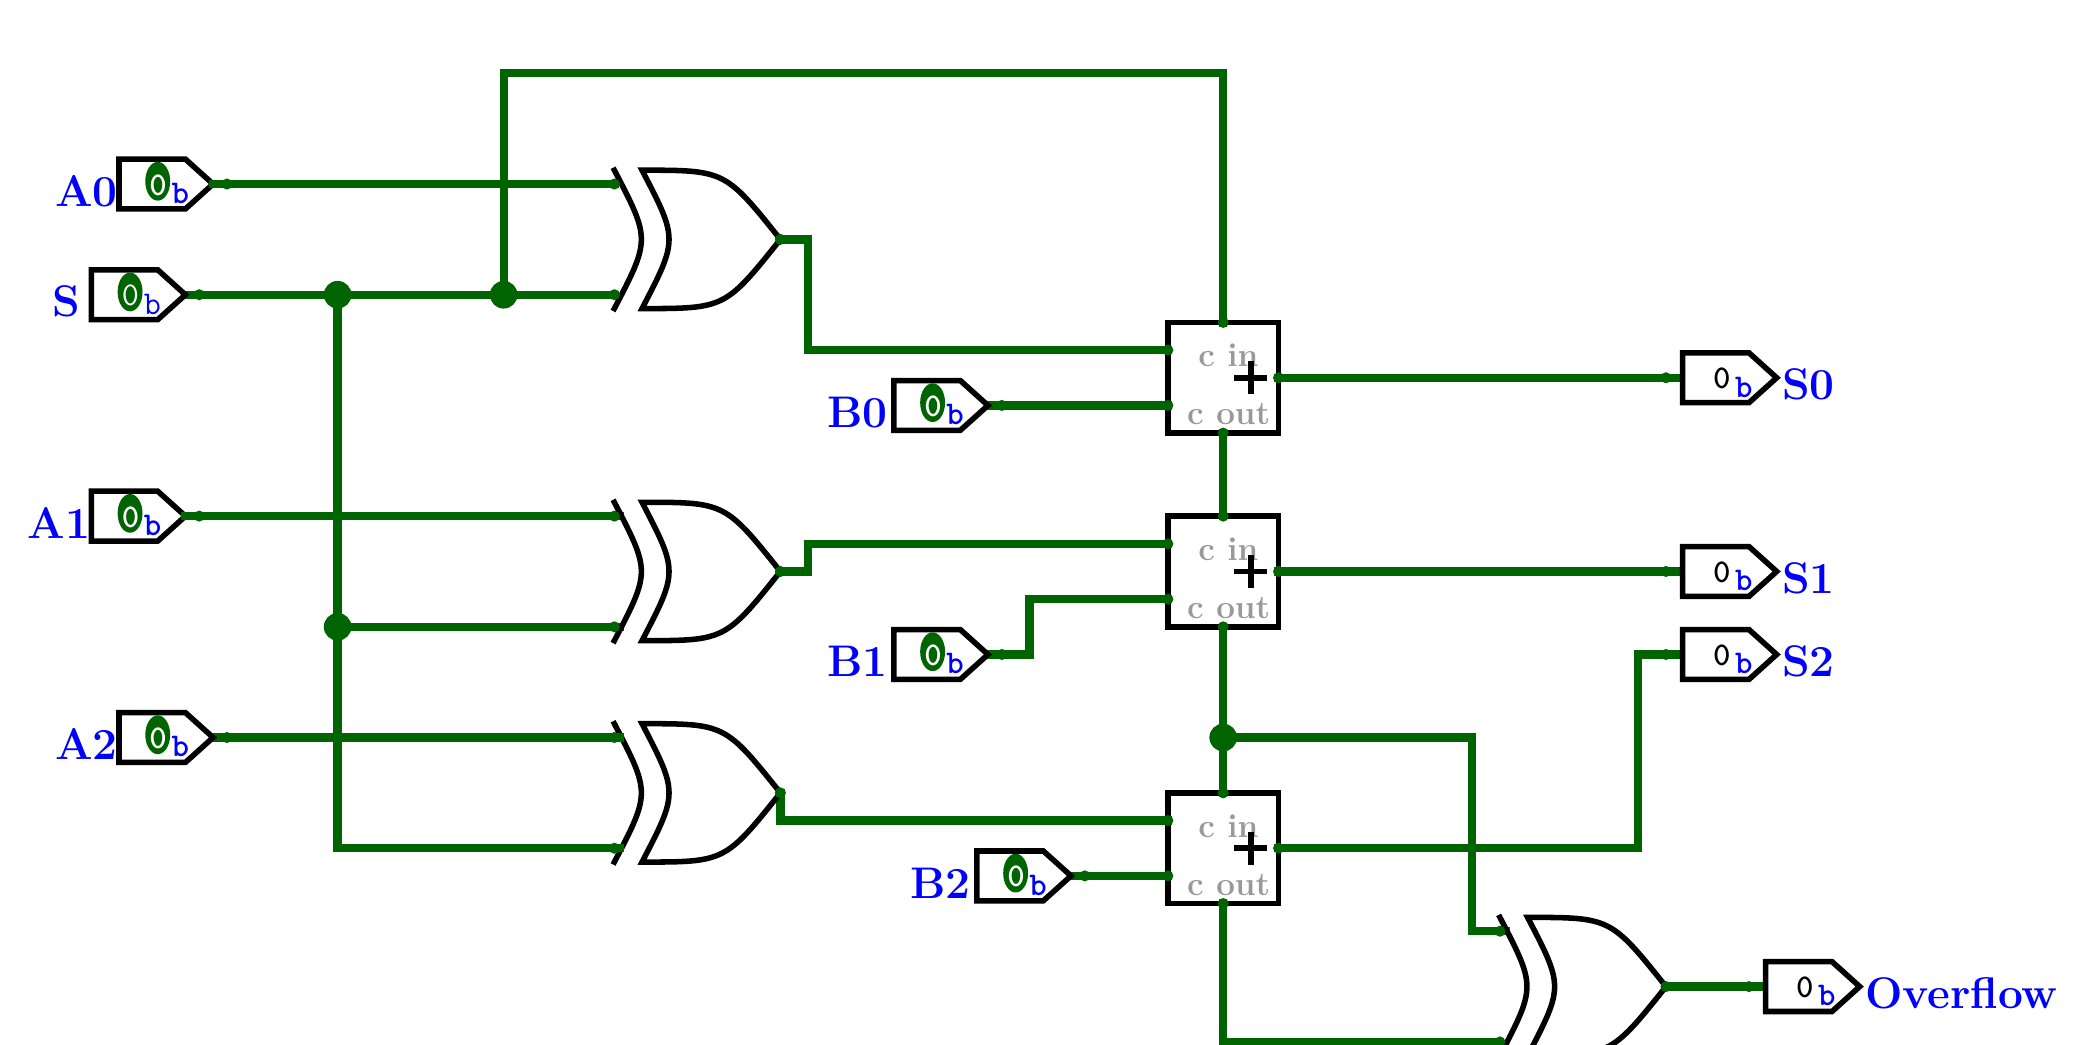
\begin{tikzpicture}[x=1pt,y=-1pt,line cap=rect]
				\def\logisimfontA#1{\fontfamily{lmr}\selectfont#1} % Use Latin Modern Roman
				\def\logisimfontB#1{\fontfamily{lmtt}\selectfont#1} % Use Latin Modern Monospace
				\definecolor{custcol_0_0_ff}{RGB}{0, 0, 255}
				\definecolor{custcol_0_64_0}{RGB}{0, 100, 0}
				\definecolor{custcol_0_0_0}{RGB}{0, 0, 0}
				\definecolor{custcol_ff_ff_ff}{RGB}{255, 255, 255}
				\definecolor{custcol_99_99_99}{RGB}{153, 153, 153}
				\draw [line width=3.0pt, custcol_0_64_0 ]  (437.0,135.0) -- (437.0,165.0) ;
				\draw [line width=3.0pt, custcol_0_64_0 ]  (597.0,335.0) -- (627.0,335.0) ;
				\draw [line width=3.0pt, custcol_0_64_0 ]  (437.0,205.0) -- (437.0,245.0) ;
				\draw [line width=3.0pt, custcol_0_64_0 ]  (277.0,265.0) -- (277.0,275.0) -- (417.0,275.0) ;
				\draw [line width=3.0pt, custcol_0_64_0 ]  (457.0,185.0) -- (597.0,185.0) ;
				\draw [line width=3.0pt, custcol_0_64_0 ]  (457.0,115.0) -- (597.0,115.0) ;
				\draw [line width=3.0pt, custcol_0_64_0 ]  (117.0,85.0) -- (117.0,205.0) ;
				\draw [line width=3.0pt, custcol_0_64_0 ]  (277.0,65.0) -- (287.0,65.0) -- (287.0,105.0) -- (417.0,105.0) ;
				\draw [line width=3.0pt, custcol_0_64_0 ]  (277.0,185.0) -- (287.0,185.0) -- (287.0,175.0) -- (417.0,175.0) ;
				\draw [line width=3.0pt, custcol_0_64_0 ]  (457.0,285.0) -- (587.0,285.0) -- (587.0,215.0) -- (597.0,215.0) ;
				\fill [line width=3.0pt, custcol_0_64_0]  (177.0,85.0) ellipse (5.0 and 5.0 );
				\fill [line width=3.0pt, custcol_0_64_0]  (437.0,245.0) ellipse (5.0 and 5.0 );
				\fill [line width=3.0pt, custcol_0_64_0]  (117.0,205.0) ellipse (5.0 and 5.0 );
				\fill [line width=3.0pt, custcol_0_64_0]  (117.0,85.0) ellipse (5.0 and 5.0 );
				\draw [line width=3.0pt, custcol_0_64_0 ]  (62.0,85.0) -- (67.0,85.0) -- (117.0,85.0) -- (177.0,85.0) -- (177.0,5.0) -- (437.0,5.0) -- (437.0,95.0) ;
				\draw [line width=2.0pt, custcol_0_0_0 ]  (52.0,94.0) -- (62.0,85.0) -- (52.0,76.0) -- (28.0,76.0) -- (28.0,94.0) -- cycle;
				\logisimfontB{\fontsize{12pt}{12pt}\selectfont\node[inner sep=0, outer sep=0, custcol_0_0_ff, anchor=base west] at  (47.0,92.0)  {b};}
				\fill [line width=2.0pt, custcol_0_64_0]  (42.0,84.0) ellipse (4.5 and 7.0 );
				\logisimfontB{\fontsize{12pt}{12pt}\selectfont\node[inner sep=0, outer sep=0, custcol_ff_ff_ff, anchor=base west] at  (39.0,89.0)  {0};}
				\logisimfontA{\fontsize{16pt}{16pt}\fontseries{bx}\selectfont\node[inner sep=0, outer sep=0, custcol_0_0_ff, anchor=base west] at  (14.0,93.0)  {S};}
				\fill [line width=2.0pt, custcol_0_64_0]  (67.0,85.0) ellipse (2.0 and 2.0 );
				\draw [line width=2.0pt, custcol_0_0_0 ]  (417.0,95.0) -- (456.0,95.0) ;
				\draw [line width=2.0pt, custcol_0_0_0 ]  (457.0,95.0) -- (457.0,134.0) ;
				\draw [line width=2.0pt, custcol_0_0_0 ]  (457.0,135.0) -- (418.0,135.0) ;
				\draw [line width=2.0pt, custcol_0_0_0 ]  (417.0,135.0) -- (417.0,96.0) ;
				\fill [line width=1.0pt, custcol_0_64_0]  (417.0,105.0) ellipse (2.0 and 2.0 );
				\fill [line width=1.0pt, custcol_0_64_0]  (417.0,125.0) ellipse (2.0 and 2.0 );
				\fill [line width=1.0pt, custcol_0_64_0]  (457.0,115.0) ellipse (2.0 and 2.0 );
				\fill [line width=1.0pt, custcol_0_64_0]  (437.0,95.0) ellipse (2.0 and 2.0 );
				\logisimfontA{\fontsize{12pt}{12pt}\selectfont\node[inner sep=0, outer sep=0, custcol_99_99_99, anchor=base west] at  (428.0,111.0)  {c in};}
				\fill [line width=1.0pt, custcol_0_64_0]  (437.0,135.0) ellipse (2.0 and 2.0 );
				\logisimfontA{\fontsize{12pt}{12pt}\selectfont\node[inner sep=0, outer sep=0, custcol_99_99_99, anchor=base west] at  (424.0,132.0)  {c out};}
				\draw [line width=2.0pt, custcol_0_0_0 ]  (442.0,115.0) -- (452.0,115.0) ;
				\draw [line width=2.0pt, custcol_0_0_0 ]  (447.0,110.0) -- (447.0,120.0) ;
				\draw [line width=2.0pt, custcol_0_0_0 ]  (417.0,165.0) -- (456.0,165.0) ;
				\draw [line width=2.0pt, custcol_0_0_0 ]  (457.0,165.0) -- (457.0,204.0) ;
				\draw [line width=2.0pt, custcol_0_0_0 ]  (457.0,205.0) -- (418.0,205.0) ;
				\draw [line width=2.0pt, custcol_0_0_0 ]  (417.0,205.0) -- (417.0,166.0) ;
				\fill [line width=1.0pt, custcol_0_64_0]  (417.0,175.0) ellipse (2.0 and 2.0 );
				\fill [line width=1.0pt, custcol_0_64_0]  (417.0,195.0) ellipse (2.0 and 2.0 );
				\fill [line width=1.0pt, custcol_0_64_0]  (457.0,185.0) ellipse (2.0 and 2.0 );
				\fill [line width=1.0pt, custcol_0_64_0]  (437.0,165.0) ellipse (2.0 and 2.0 );
				\logisimfontA{\fontsize{12pt}{12pt}\selectfont\node[inner sep=0, outer sep=0, custcol_99_99_99, anchor=base west] at  (428.0,181.0)  {c in};}
				\fill [line width=1.0pt, custcol_0_64_0]  (437.0,205.0) ellipse (2.0 and 2.0 );
				\logisimfontA{\fontsize{12pt}{12pt}\selectfont\node[inner sep=0, outer sep=0, custcol_99_99_99, anchor=base west] at  (424.0,202.0)  {c out};}
				\draw [line width=2.0pt, custcol_0_0_0 ]  (442.0,185.0) -- (452.0,185.0) ;
				\draw [line width=2.0pt, custcol_0_0_0 ]  (447.0,180.0) -- (447.0,190.0) ;
				\draw [line width=2.0pt, custcol_0_0_0 ]  (277.0,265.0) .. controls  (257.0,240.0)  ..  (227.0,240.0) .. controls  (240.0,265.0)  ..  (227.0,290.0) .. controls  (257.0,290.0)  ..  (277.0,265.0) -- cycle ;
				\draw [line width=2.0pt, custcol_0_0_0 ]  (217.0,240.0) .. controls  (230.0,265.0)  ..  (217.0,290.0) ;
				\fill [line width=2.0pt, custcol_0_64_0]  (277.0,265.0) ellipse (2.0 and 2.0 );
				\fill [line width=2.0pt, custcol_0_64_0]  (217.0,245.0) ellipse (2.0 and 2.0 );
				\fill [line width=2.0pt, custcol_0_64_0]  (217.0,285.0) ellipse (2.0 and 2.0 );
				\draw [line width=2.0pt, custcol_0_0_0 ]  (417.0,265.0) -- (456.0,265.0) ;
				\draw [line width=2.0pt, custcol_0_0_0 ]  (457.0,265.0) -- (457.0,304.0) ;
				\draw [line width=2.0pt, custcol_0_0_0 ]  (457.0,305.0) -- (418.0,305.0) ;
				\draw [line width=2.0pt, custcol_0_0_0 ]  (417.0,305.0) -- (417.0,266.0) ;
				\fill [line width=1.0pt, custcol_0_64_0]  (417.0,275.0) ellipse (2.0 and 2.0 );
				\fill [line width=1.0pt, custcol_0_64_0]  (417.0,295.0) ellipse (2.0 and 2.0 );
				\fill [line width=1.0pt, custcol_0_64_0]  (457.0,285.0) ellipse (2.0 and 2.0 );
				\fill [line width=1.0pt, custcol_0_64_0]  (437.0,265.0) ellipse (2.0 and 2.0 );
				\logisimfontA{\fontsize{12pt}{12pt}\selectfont\node[inner sep=0, outer sep=0, custcol_99_99_99, anchor=base west] at  (428.0,281.0)  {c in};}
				\fill [line width=1.0pt, custcol_0_64_0]  (437.0,305.0) ellipse (2.0 and 2.0 );
				\logisimfontA{\fontsize{12pt}{12pt}\selectfont\node[inner sep=0, outer sep=0, custcol_99_99_99, anchor=base west] at  (424.0,302.0)  {c out};}
				\draw [line width=2.0pt, custcol_0_0_0 ]  (442.0,285.0) -- (452.0,285.0) ;
				\draw [line width=2.0pt, custcol_0_0_0 ]  (447.0,280.0) -- (447.0,290.0) ;
				\draw [line width=2.0pt, custcol_0_0_0 ]  (62.0,54.0) -- (72.0,45.0) -- (62.0,36.0) -- (38.0,36.0) -- (38.0,54.0) -- cycle;
				\logisimfontB{\fontsize{12pt}{12pt}\selectfont\node[inner sep=0, outer sep=0, custcol_0_0_ff, anchor=base west] at  (57.0,52.0)  {b};}
				\fill [line width=2.0pt, custcol_0_64_0]  (52.0,44.0) ellipse (4.5 and 7.0 );
				\logisimfontB{\fontsize{12pt}{12pt}\selectfont\node[inner sep=0, outer sep=0, custcol_ff_ff_ff, anchor=base west] at  (49.0,49.0)  {0};}
				\logisimfontA{\fontsize{16pt}{16pt}\fontseries{bx}\selectfont\node[inner sep=0, outer sep=0, custcol_0_0_ff, anchor=base west] at  (15.0,53.0)  {A0};}
				\fill [line width=2.0pt, custcol_0_64_0]  (77.0,45.0) ellipse (2.0 and 2.0 );
				\draw [line width=2.0pt, custcol_0_0_0 ]  (52.0,174.0) -- (62.0,165.0) -- (52.0,156.0) -- (28.0,156.0) -- (28.0,174.0) -- cycle;
				\logisimfontB{\fontsize{12pt}{12pt}\selectfont\node[inner sep=0, outer sep=0, custcol_0_0_ff, anchor=base west] at  (47.0,172.0)  {b};}
				\fill [line width=2.0pt, custcol_0_64_0]  (42.0,164.0) ellipse (4.5 and 7.0 );
				\logisimfontB{\fontsize{12pt}{12pt}\selectfont\node[inner sep=0, outer sep=0, custcol_ff_ff_ff, anchor=base west] at  (39.0,169.0)  {0};}
				\logisimfontA{\fontsize{16pt}{16pt}\fontseries{bx}\selectfont\node[inner sep=0, outer sep=0, custcol_0_0_ff, anchor=base west] at  (5.0,173.0)  {A1};}
				\fill [line width=2.0pt, custcol_0_64_0]  (67.0,165.0) ellipse (2.0 and 2.0 );
				\draw [line width=3.0pt, custcol_0_64_0 ]  (72.0,245.0) -- (77.0,245.0) -- (217.0,245.0) -- (219.0,245.0) ;
				\draw [line width=2.0pt, custcol_0_0_0 ]  (62.0,254.0) -- (72.0,245.0) -- (62.0,236.0) -- (38.0,236.0) -- (38.0,254.0) -- cycle;
				\logisimfontB{\fontsize{12pt}{12pt}\selectfont\node[inner sep=0, outer sep=0, custcol_0_0_ff, anchor=base west] at  (57.0,252.0)  {b};}
				\fill [line width=2.0pt, custcol_0_64_0]  (52.0,244.0) ellipse (4.5 and 7.0 );
				\logisimfontB{\fontsize{12pt}{12pt}\selectfont\node[inner sep=0, outer sep=0, custcol_ff_ff_ff, anchor=base west] at  (49.0,249.0)  {0};}
				\logisimfontA{\fontsize{16pt}{16pt}\fontseries{bx}\selectfont\node[inner sep=0, outer sep=0, custcol_0_0_ff, anchor=base west] at  (15.0,253.0)  {A2};}
				\fill [line width=2.0pt, custcol_0_64_0]  (77.0,245.0) ellipse (2.0 and 2.0 );
				\draw [line width=3.0pt, custcol_0_64_0 ]  (352.0,125.0) -- (357.0,125.0) -- (417.0,125.0) ;
				\draw [line width=2.0pt, custcol_0_0_0 ]  (342.0,134.0) -- (352.0,125.0) -- (342.0,116.0) -- (318.0,116.0) -- (318.0,134.0) -- cycle;
				\logisimfontB{\fontsize{12pt}{12pt}\selectfont\node[inner sep=0, outer sep=0, custcol_0_0_ff, anchor=base west] at  (337.0,132.0)  {b};}
				\fill [line width=2.0pt, custcol_0_64_0]  (332.0,124.0) ellipse (4.5 and 7.0 );
				\logisimfontB{\fontsize{12pt}{12pt}\selectfont\node[inner sep=0, outer sep=0, custcol_ff_ff_ff, anchor=base west] at  (329.0,129.0)  {0};}
				\logisimfontA{\fontsize{16pt}{16pt}\fontseries{bx}\selectfont\node[inner sep=0, outer sep=0, custcol_0_0_ff, anchor=base west] at  (294.0,133.0)  {B0};}
				\fill [line width=2.0pt, custcol_0_64_0]  (357.0,125.0) ellipse (2.0 and 2.0 );
				\draw [line width=3.0pt, custcol_0_64_0 ]  (352.0,215.0) -- (357.0,215.0) -- (367.0,215.0) -- (367.0,195.0) -- (417.0,195.0) ;
				\draw [line width=2.0pt, custcol_0_0_0 ]  (342.0,224.0) -- (352.0,215.0) -- (342.0,206.0) -- (318.0,206.0) -- (318.0,224.0) -- cycle;
				\logisimfontB{\fontsize{12pt}{12pt}\selectfont\node[inner sep=0, outer sep=0, custcol_0_0_ff, anchor=base west] at  (337.0,222.0)  {b};}
				\fill [line width=2.0pt, custcol_0_64_0]  (332.0,214.0) ellipse (4.5 and 7.0 );
				\logisimfontB{\fontsize{12pt}{12pt}\selectfont\node[inner sep=0, outer sep=0, custcol_ff_ff_ff, anchor=base west] at  (329.0,219.0)  {0};}
				\logisimfontA{\fontsize{16pt}{16pt}\fontseries{bx}\selectfont\node[inner sep=0, outer sep=0, custcol_0_0_ff, anchor=base west] at  (294.0,223.0)  {B1};}
				\fill [line width=2.0pt, custcol_0_64_0]  (357.0,215.0) ellipse (2.0 and 2.0 );
				\draw [line width=3.0pt, custcol_0_64_0 ]  (382.0,295.0) -- (387.0,295.0) -- (417.0,295.0) ;
				\draw [line width=2.0pt, custcol_0_0_0 ]  (372.0,304.0) -- (382.0,295.0) -- (372.0,286.0) -- (348.0,286.0) -- (348.0,304.0) -- cycle;
				\logisimfontB{\fontsize{12pt}{12pt}\selectfont\node[inner sep=0, outer sep=0, custcol_0_0_ff, anchor=base west] at  (367.0,302.0)  {b};}
				\fill [line width=2.0pt, custcol_0_64_0]  (362.0,294.0) ellipse (4.5 and 7.0 );
				\logisimfontB{\fontsize{12pt}{12pt}\selectfont\node[inner sep=0, outer sep=0, custcol_ff_ff_ff, anchor=base west] at  (359.0,299.0)  {0};}
				\logisimfontA{\fontsize{16pt}{16pt}\fontseries{bx}\selectfont\node[inner sep=0, outer sep=0, custcol_0_0_ff, anchor=base west] at  (324.0,303.0)  {B2};}
				\fill [line width=2.0pt, custcol_0_64_0]  (387.0,295.0) ellipse (2.0 and 2.0 );
				\draw [line width=3.0pt, custcol_0_64_0 ]  (601.0,185.0) -- (598.0,185.0) ;
				\draw [line width=2.0pt, custcol_0_0_0 ]  (627.0,176.0) -- (637.0,185.0) -- (627.0,194.0) -- (603.0,194.0) -- (603.0,176.0) -- cycle;
				\logisimfontB{\fontsize{12pt}{12pt}\selectfont\node[inner sep=0, outer sep=0, custcol_0_0_ff, anchor=base west] at  (622.0,192.0)  {b};}
				\logisimfontB{\fontsize{12pt}{12pt}\selectfont\node[inner sep=0, outer sep=0, custcol_0_0_0, anchor=base west] at  (614.0,189.0)  {0};}
				\logisimfontA{\fontsize{16pt}{16pt}\fontseries{bx}\selectfont\node[inner sep=0, outer sep=0, custcol_0_0_ff, anchor=base west] at  (639.0,193.0)  {S1};}
				\fill [line width=2.0pt, custcol_0_64_0]  (597.0,185.0) ellipse (2.0 and 2.0 );
				\draw [line width=3.0pt, custcol_0_64_0 ]  (437.0,265.0) -- (437.0,245.0) -- (527.0,245.0) -- (527.0,315.0) -- (537.0,315.0) -- (539.0,315.0) ;
				\draw [line width=3.0pt, custcol_0_64_0 ]  (437.0,305.0) -- (437.0,355.0) -- (537.0,355.0) -- (537.0,355.0) ;
				\draw [line width=2.0pt, custcol_0_0_0 ]  (597.0,335.0) .. controls  (577.0,310.0)  ..  (547.0,310.0) .. controls  (560.0,335.0)  ..  (547.0,360.0) .. controls  (577.0,360.0)  ..  (597.0,335.0) -- cycle ;
				\draw [line width=2.0pt, custcol_0_0_0 ]  (537.0,310.0) .. controls  (550.0,335.0)  ..  (537.0,360.0) ;
				\fill [line width=2.0pt, custcol_0_64_0]  (597.0,335.0) ellipse (2.0 and 2.0 );
				\fill [line width=2.0pt, custcol_0_64_0]  (537.0,315.0) ellipse (2.0 and 2.0 );
				\fill [line width=2.0pt, custcol_0_64_0]  (537.0,355.0) ellipse (2.0 and 2.0 );
				\draw [line width=3.0pt, custcol_0_64_0 ]  (631.0,335.0) -- (628.0,335.0) ;
				\draw [line width=2.0pt, custcol_0_0_0 ]  (657.0,326.0) -- (667.0,335.0) -- (657.0,344.0) -- (633.0,344.0) -- (633.0,326.0) -- cycle;
				\logisimfontB{\fontsize{12pt}{12pt}\selectfont\node[inner sep=0, outer sep=0, custcol_0_0_ff, anchor=base west] at  (652.0,342.0)  {b};}
				\logisimfontB{\fontsize{12pt}{12pt}\selectfont\node[inner sep=0, outer sep=0, custcol_0_0_0, anchor=base west] at  (644.0,339.0)  {0};}
				\logisimfontA{\fontsize{16pt}{16pt}\fontseries{bx}\selectfont\node[inner sep=0, outer sep=0, custcol_0_0_ff, anchor=base west] at  (669.0,343.0)  {Overflow};}
				\fill [line width=2.0pt, custcol_0_64_0]  (627.0,335.0) ellipse (2.0 and 2.0 );
				\draw [line width=3.0pt, custcol_0_64_0 ]  (601.0,115.0) -- (598.0,115.0) ;
				\draw [line width=2.0pt, custcol_0_0_0 ]  (627.0,106.0) -- (637.0,115.0) -- (627.0,124.0) -- (603.0,124.0) -- (603.0,106.0) -- cycle;
				\logisimfontB{\fontsize{12pt}{12pt}\selectfont\node[inner sep=0, outer sep=0, custcol_0_0_ff, anchor=base west] at  (622.0,122.0)  {b};}
				\logisimfontB{\fontsize{12pt}{12pt}\selectfont\node[inner sep=0, outer sep=0, custcol_0_0_0, anchor=base west] at  (614.0,119.0)  {0};}
				\logisimfontA{\fontsize{16pt}{16pt}\fontseries{bx}\selectfont\node[inner sep=0, outer sep=0, custcol_0_0_ff, anchor=base west] at  (639.0,123.0)  {S0};}
				\fill [line width=2.0pt, custcol_0_64_0]  (597.0,115.0) ellipse (2.0 and 2.0 );
				\draw [line width=3.0pt, custcol_0_64_0 ]  (601.0,215.0) -- (598.0,215.0) ;
				\draw [line width=2.0pt, custcol_0_0_0 ]  (627.0,206.0) -- (637.0,215.0) -- (627.0,224.0) -- (603.0,224.0) -- (603.0,206.0) -- cycle;
				\logisimfontB{\fontsize{12pt}{12pt}\selectfont\node[inner sep=0, outer sep=0, custcol_0_0_ff, anchor=base west] at  (622.0,222.0)  {b};}
				\logisimfontB{\fontsize{12pt}{12pt}\selectfont\node[inner sep=0, outer sep=0, custcol_0_0_0, anchor=base west] at  (614.0,219.0)  {0};}
				\logisimfontA{\fontsize{16pt}{16pt}\fontseries{bx}\selectfont\node[inner sep=0, outer sep=0, custcol_0_0_ff, anchor=base west] at  (639.0,223.0)  {S2};}
				\fill [line width=2.0pt, custcol_0_64_0]  (597.0,215.0) ellipse (2.0 and 2.0 );
				\draw [line width=3.0pt, custcol_0_64_0 ]  (72.0,45.0) -- (77.0,45.0) -- (217.0,45.0) -- (217.0,45.0) ;
				\draw [line width=3.0pt, custcol_0_64_0 ]  (177.0,85.0) -- (217.0,85.0) -- (217.0,85.0) ;
				\draw [line width=2.0pt, custcol_0_0_0 ]  (277.0,65.0) .. controls  (257.0,40.0)  ..  (227.0,40.0) .. controls  (240.0,65.0)  ..  (227.0,90.0) .. controls  (257.0,90.0)  ..  (277.0,65.0) -- cycle ;
				\draw [line width=2.0pt, custcol_0_0_0 ]  (217.0,40.0) .. controls  (230.0,65.0)  ..  (217.0,90.0) ;
				\fill [line width=2.0pt, custcol_0_64_0]  (277.0,65.0) ellipse (2.0 and 2.0 );
				\fill [line width=2.0pt, custcol_0_64_0]  (217.0,45.0) ellipse (2.0 and 2.0 );
				\fill [line width=2.0pt, custcol_0_64_0]  (217.0,85.0) ellipse (2.0 and 2.0 );
				\draw [line width=3.0pt, custcol_0_64_0 ]  (62.0,165.0) -- (67.0,165.0) -- (217.0,165.0) -- (219.0,165.0) ;
				\draw [line width=3.0pt, custcol_0_64_0 ]  (219.0,285.0) -- (217.0,285.0) -- (117.0,285.0) -- (117.0,205.0) -- (217.0,205.0) -- (219.0,205.0) ;
				\draw [line width=2.0pt, custcol_0_0_0 ]  (277.0,185.0) .. controls  (257.0,160.0)  ..  (227.0,160.0) .. controls  (240.0,185.0)  ..  (227.0,210.0) .. controls  (257.0,210.0)  ..  (277.0,185.0) -- cycle ;
				\draw [line width=2.0pt, custcol_0_0_0 ]  (217.0,160.0) .. controls  (230.0,185.0)  ..  (217.0,210.0) ;
				\fill [line width=2.0pt, custcol_0_64_0]  (277.0,185.0) ellipse (2.0 and 2.0 );
				\fill [line width=2.0pt, custcol_0_64_0]  (217.0,165.0) ellipse (2.0 and 2.0 );
				\fill [line width=2.0pt, custcol_0_64_0]  (217.0,205.0) ellipse (2.0 and 2.0 );
			\end{tikzpicture}}
		\caption{A simple 3 bit adder/subtractor circuit}
	\end{figure}
\end{examp}
\subsection{A Priority Encoder/Comparator}
\begin{examp}
	\textbf{Design a Circuit to Compare two 2-bit Numbers}\\
	Given \( A = A_1A_0 \) and \( B = B_1B_0 \), design a circuit that will
	output 0 if the two numbers are equal, 1 otherwise.

	You can only use 2 input XOR gates (limitless), one OR gate, and one
	INVERTER gate.

	The solution for this one also lies in the XOR gate. You simply only need
	Three XOR gates to compare the two numbers. The output of the XOR gates
	will be 0 if the two numbers are equal, and 1 otherwise. The OR gate
	will then be used to combine the outputs of the XOR gates. The INVERTER
	is not needed as we are outputting 0 when the condition is true.
	\begin{figure}[H]
		\resizebox{15cm}{!}{
			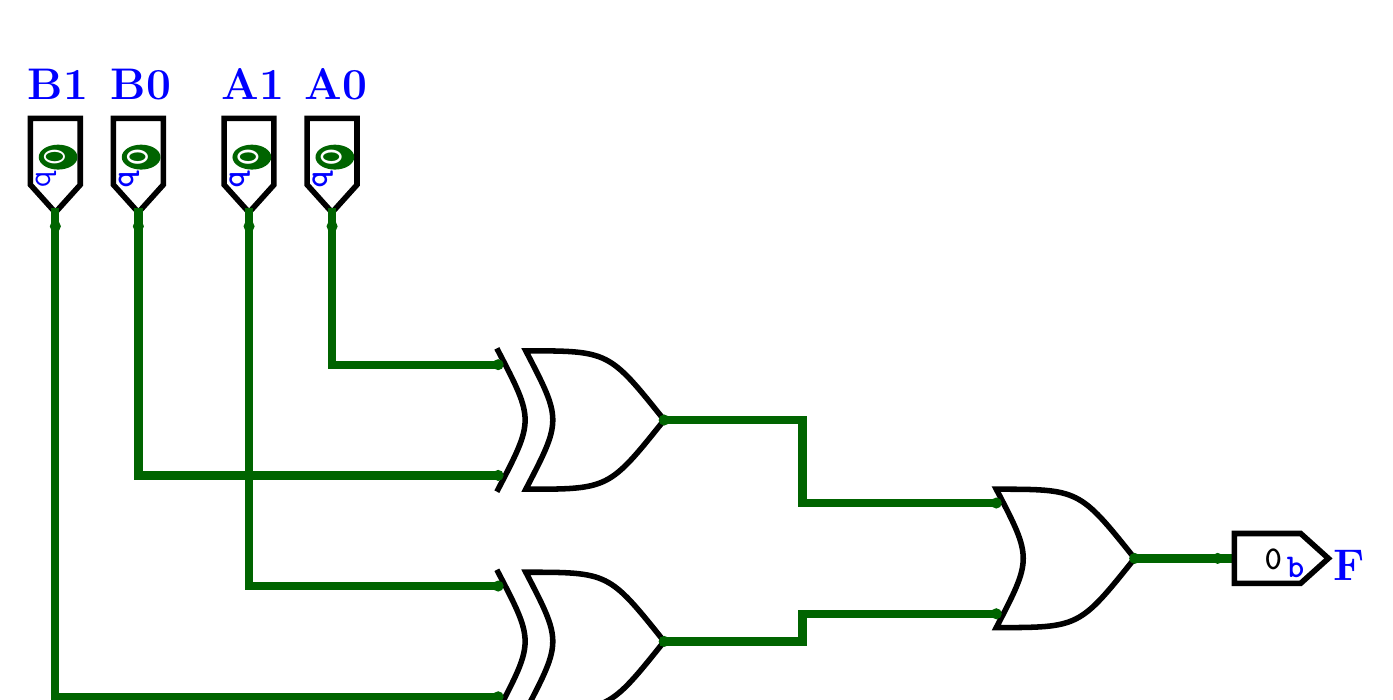
\begin{tikzpicture}[x=1pt,y=-1pt,line cap=rect]
				\def\logisimfontA#1{\fontfamily{lmr}\selectfont#1} % Use Latin Modern Roman
				\def\logisimfontB#1{\fontfamily{lmtt}\selectfont#1} % Use Latin Modern Monospace
				\definecolor{custcol_0_0_ff}{RGB}{0, 0, 255}
				\definecolor{custcol_0_64_0}{RGB}{0, 100, 0}
				\definecolor{custcol_0_0_0}{RGB}{0, 0, 0}
				\definecolor{custcol_ff_ff_ff}{RGB}{255, 255, 255}
				\draw [line width=3.0pt, custcol_0_64_0 ]  (405.0,188.0) -- (435.0,188.0) ;
				\draw [line width=2.0pt, custcol_0_0_0 ]  (6.0,53.0) -- (15.0,63.0) -- (24.0,53.0) -- (24.0,29.0) -- (6.0,29.0) -- cycle;
				\logisimfontB{\fontsize{12pt}{12pt}\selectfont\node[inner sep=0, outer sep=0, custcol_0_0_ff, anchor=base west, rotate=-90.0] at  (8.0,48.0)  {b};}
				\fill [line width=2.0pt, custcol_0_64_0, rotate around={90: (16.0,43.0) }]  (16.0,43.0) ellipse (4.5 and 7.0 );
				\logisimfontB{\fontsize{12pt}{12pt}\selectfont\node[inner sep=0, outer sep=0, custcol_ff_ff_ff, anchor=base west, rotate=-90.0] at  (11.0,40.0)  {0};}
				\logisimfontA{\fontsize{16pt}{16pt}\fontseries{bx}\selectfont\node[inner sep=0, outer sep=0, custcol_0_0_ff, anchor=base west] at  (5.0,22.0)  {B1};}
				\fill [line width=2.0pt, custcol_0_64_0]  (15.0,68.0) ellipse (2.0 and 2.0 );
				\draw [line width=2.0pt, custcol_0_0_0 ]  (36.0,53.0) -- (45.0,63.0) -- (54.0,53.0) -- (54.0,29.0) -- (36.0,29.0) -- cycle;
				\logisimfontB{\fontsize{12pt}{12pt}\selectfont\node[inner sep=0, outer sep=0, custcol_0_0_ff, anchor=base west, rotate=-90.0] at  (38.0,48.0)  {b};}
				\fill [line width=2.0pt, custcol_0_64_0, rotate around={90: (46.0,43.0) }]  (46.0,43.0) ellipse (4.5 and 7.0 );
				\logisimfontB{\fontsize{12pt}{12pt}\selectfont\node[inner sep=0, outer sep=0, custcol_ff_ff_ff, anchor=base west, rotate=-90.0] at  (41.0,40.0)  {0};}
				\logisimfontA{\fontsize{16pt}{16pt}\fontseries{bx}\selectfont\node[inner sep=0, outer sep=0, custcol_0_0_ff, anchor=base west] at  (35.0,22.0)  {B0};}
				\fill [line width=2.0pt, custcol_0_64_0]  (45.0,68.0) ellipse (2.0 and 2.0 );
				\draw [line width=2.0pt, custcol_0_0_0 ]  (76.0,53.0) -- (85.0,63.0) -- (94.0,53.0) -- (94.0,29.0) -- (76.0,29.0) -- cycle;
				\logisimfontB{\fontsize{12pt}{12pt}\selectfont\node[inner sep=0, outer sep=0, custcol_0_0_ff, anchor=base west, rotate=-90.0] at  (78.0,48.0)  {b};}
				\fill [line width=2.0pt, custcol_0_64_0, rotate around={90: (86.0,43.0) }]  (86.0,43.0) ellipse (4.5 and 7.0 );
				\logisimfontB{\fontsize{12pt}{12pt}\selectfont\node[inner sep=0, outer sep=0, custcol_ff_ff_ff, anchor=base west, rotate=-90.0] at  (81.0,40.0)  {0};}
				\logisimfontA{\fontsize{16pt}{16pt}\fontseries{bx}\selectfont\node[inner sep=0, outer sep=0, custcol_0_0_ff, anchor=base west] at  (75.0,22.0)  {A1};}
				\fill [line width=2.0pt, custcol_0_64_0]  (85.0,68.0) ellipse (2.0 and 2.0 );
				\draw [line width=2.0pt, custcol_0_0_0 ]  (106.0,53.0) -- (115.0,63.0) -- (124.0,53.0) -- (124.0,29.0) -- (106.0,29.0) -- cycle;
				\logisimfontB{\fontsize{12pt}{12pt}\selectfont\node[inner sep=0, outer sep=0, custcol_0_0_ff, anchor=base west, rotate=-90.0] at  (108.0,48.0)  {b};}
				\fill [line width=2.0pt, custcol_0_64_0, rotate around={90: (116.0,43.0) }]  (116.0,43.0) ellipse (4.5 and 7.0 );
				\logisimfontB{\fontsize{12pt}{12pt}\selectfont\node[inner sep=0, outer sep=0, custcol_ff_ff_ff, anchor=base west, rotate=-90.0] at  (111.0,40.0)  {0};}
				\logisimfontA{\fontsize{16pt}{16pt}\fontseries{bx}\selectfont\node[inner sep=0, outer sep=0, custcol_0_0_ff, anchor=base west] at  (105.0,22.0)  {A0};}
				\fill [line width=2.0pt, custcol_0_64_0]  (115.0,68.0) ellipse (2.0 and 2.0 );
				\draw [line width=3.0pt, custcol_0_64_0 ]  (115.0,63.0) -- (115.0,68.0) -- (115.0,118.0) -- (175.0,118.0) -- (175.0,118.0) ;
				\draw [line width=3.0pt, custcol_0_64_0 ]  (45.0,63.0) -- (45.0,68.0) -- (45.0,158.0) -- (175.0,158.0) -- (175.0,158.0) ;
				\draw [line width=2.0pt, custcol_0_0_0 ]  (235.0,138.0) .. controls  (215.0,113.0)  ..  (185.0,113.0) .. controls  (198.0,138.0)  ..  (185.0,163.0) .. controls  (215.0,163.0)  ..  (235.0,138.0) -- cycle ;
				\draw [line width=2.0pt, custcol_0_0_0 ]  (175.0,113.0) .. controls  (188.0,138.0)  ..  (175.0,163.0) ;
				\fill [line width=2.0pt, custcol_0_64_0]  (235.0,138.0) ellipse (2.0 and 2.0 );
				\fill [line width=2.0pt, custcol_0_64_0]  (175.0,118.0) ellipse (2.0 and 2.0 );
				\fill [line width=2.0pt, custcol_0_64_0]  (175.0,158.0) ellipse (2.0 and 2.0 );
				\draw [line width=3.0pt, custcol_0_64_0 ]  (85.0,63.0) -- (85.0,68.0) -- (85.0,198.0) -- (175.0,198.0) -- (175.0,198.0) ;
				\draw [line width=3.0pt, custcol_0_64_0 ]  (15.0,63.0) -- (15.0,68.0) -- (15.0,238.0) -- (175.0,238.0) -- (175.0,238.0) ;
				\draw [line width=2.0pt, custcol_0_0_0 ]  (235.0,218.0) .. controls  (215.0,193.0)  ..  (185.0,193.0) .. controls  (198.0,218.0)  ..  (185.0,243.0) .. controls  (215.0,243.0)  ..  (235.0,218.0) -- cycle ;
				\draw [line width=2.0pt, custcol_0_0_0 ]  (175.0,193.0) .. controls  (188.0,218.0)  ..  (175.0,243.0) ;
				\fill [line width=2.0pt, custcol_0_64_0]  (235.0,218.0) ellipse (2.0 and 2.0 );
				\fill [line width=2.0pt, custcol_0_64_0]  (175.0,198.0) ellipse (2.0 and 2.0 );
				\fill [line width=2.0pt, custcol_0_64_0]  (175.0,238.0) ellipse (2.0 and 2.0 );
				\draw [line width=3.0pt, custcol_0_64_0 ]  (235.0,138.0) -- (285.0,138.0) -- (285.0,168.0) -- (355.0,168.0) -- (355.0,168.0) ;
				\draw [line width=3.0pt, custcol_0_64_0 ]  (235.0,218.0) -- (285.0,218.0) -- (285.0,208.0) -- (355.0,208.0) -- (355.0,208.0) ;
				\draw [line width=2.0pt, custcol_0_0_0 ]  (405.0,188.0) .. controls  (385.0,163.0)  ..  (355.0,163.0) .. controls  (368.0,188.0)  ..  (355.0,213.0) .. controls  (385.0,213.0)  ..  (405.0,188.0) -- cycle ;
				\fill [line width=2.0pt, custcol_0_64_0]  (405.0,188.0) ellipse (2.0 and 2.0 );
				\fill [line width=2.0pt, custcol_0_64_0]  (355.0,168.0) ellipse (2.0 and 2.0 );
				\fill [line width=2.0pt, custcol_0_64_0]  (355.0,208.0) ellipse (2.0 and 2.0 );
				\draw [line width=3.0pt, custcol_0_64_0 ]  (439.0,188.0) -- (436.0,188.0) ;
				\draw [line width=2.0pt, custcol_0_0_0 ]  (465.0,179.0) -- (475.0,188.0) -- (465.0,197.0) -- (441.0,197.0) -- (441.0,179.0) -- cycle;
				\logisimfontB{\fontsize{12pt}{12pt}\selectfont\node[inner sep=0, outer sep=0, custcol_0_0_ff, anchor=base west] at  (460.0,195.0)  {b};}
				\logisimfontB{\fontsize{12pt}{12pt}\selectfont\node[inner sep=0, outer sep=0, custcol_0_0_0, anchor=base west] at  (452.0,192.0)  {0};}
				\logisimfontA{\fontsize{16pt}{16pt}\fontseries{bx}\selectfont\node[inner sep=0, outer sep=0, custcol_0_0_ff, anchor=base west] at  (477.0,196.0)  {F};}
				\fill [line width=2.0pt, custcol_0_64_0]  (435.0,188.0) ellipse (2.0 and 2.0 );
			\end{tikzpicture}}
		\caption{A simple 2 bit number comparator}
	\end{figure}
\end{examp}

\section{Exam 3: Sequential Circuits}
\subsection{Topical Guide Objectives}
\begin{enumerate}
	\item Understand and derive Latches and Flip-Flops.
	\item Know the difference between a serial and parallel operation.
	\item Be able to implement different Flip-Flops in terms of other Flip-Flops.
	\item Understand the concept of timing diagrams for edge-triggered vs
	      level triggered devices and draw them.
	\item Derive the next-state and output equations for a given state
	      diagram.
	\item Define shift operations and their applications (Sequential Multiplier)
	\item Be able to design a Mealy and Moore State Machine from a given
	      description.
	\item Be able to walk through the operation of a sequential circuit such
	      as a counter or a shift register and multiplier.
	\item Define a PLA and its applications. Be able to design a PLA from a
	      given truth table as well as derive the equations from a given
	      circuit.
\end{enumerate}
\subsection{Vocabulary}
\begin{itemize}
	\item \textbf{Sequential Circuit:} A circuit that has memory.
	\item \textbf{State:} The current condition of the circuit.
	\item \textbf{State Diagram:} A diagram that shows the states of a
	      sequential circuit and the transitions between them.
	\item \textbf{State Table:} A table that shows the current state, the
	      inputs, the next state, and the outputs.
	\item \textbf{Latch:} A circuit that can store one bit of information.
	\item \textbf{Flip-Flop:} A circuit that has two stable states and can
	      be used to store one bit of information.
	\item \textbf{Clock:} A signal that is used to synchronize the
	      operation of a sequential circuit.
	\item \textbf{Edge-Triggered:} A circuit that changes state on the
	      rising or falling edge of a clock signal.
	\item \textbf{Level-Triggered:} A circuit that changes state when the
	      clock signal is high or low.
\end{itemize}
\subsection{Shifting Operations}
\begin{itemize}
	\item \textbf{Shift Left:} Move all bits to the left and fill in the
	      rightmost bit with a 0. This is equivalent to multiplying by 2.
	\item \textbf{Shift Right:} Move all bits to the right and fill in the
	      leftmost bit with a 0. This is equivalent to dividing by 2.
\end{itemize}
\begin{examp}
	\begin{itemize}
		\item What is the arithemtic result of shifiting a loaded register by two steps
		      to the left?

		      This is equivalent to multiplying the number by \(2^2 = 4\).

		\item What is the arithmetic result of shifting a loaded register by four steps
		      to the right?

		      This is equivalent to dividing the number by \(2^4 = 16\).
	\end{itemize}
\end{examp}
\subsection{Serial vs Parallel Operations}
\begin{itemize}
	\item \textbf{Serial:} Data is transmitted one bit at a time.
	\item \textbf{Parallel:} Data is transmitted multiple bits at a time.
\end{itemize}
\begin{examp}
	\begin{itemize}
		\item How many clock pulses does it take to serially load an 8-bit register?

		      It takes 8 clock pulses to serially load an 8-bit register.
		\item How many clock pulses does it take to parallel load an 8-bit register?

		      It takes 1 clock pulse to parallel load an 8-bit register.
	\end{itemize}
\end{examp}
\subsection{Latches and Flip-Flops}
\subsubsection{The SR Latch}
\begin{itemize}
	\item The SR Latch is the simplest form of a latch.
	\item It has two inputs, S (Set) and R (Reset).
	\item It has two outputs, Q and \(\closure{Q}\).
	      \begin{figure}[H]
		      \centering
		      \begin{tabular}{|c|c|c|c|}
			      \hline
			      S & R & Q & \(\closure{Q}\) \\
			      \hline
			      0 & 0 & Q & \(\closure{Q}\) \\
			      0 & 1 & 0 & 1               \\
			      1 & 0 & 1 & 0               \\
			      1 & 1 & X & X               \\
			      \hline
		      \end{tabular}
		      \caption{The Truth Table for an SR Latch}
	      \end{figure}
	\item The major disadvantage is that the \(S = 1\) and \(R = 1\) state is
	      undefined. This can be remedied by using a gated SR latch.

\end{itemize}
\subsubsection{The Gated SR Latch}
\begin{itemize}
	\item The Gated SR Latch is an SR Latch with an additional enable input.
	\item It has three inputs, S (Set), R (Reset), and E (Enable).
	\item It has two outputs, Q and \(\closure{Q}\).
	      \begin{figure}[H]
		      \centering
		      \begin{tabular}{|c|c|c|c|c|}
			      \hline
			      S & R & E & Q & \(\closure{Q}\) \\
			      \hline
			      0 & 0 & 0 & Q & \(\closure{Q}\) \\
			      0 & 0 & 1 & Q & \(\closure{Q}\) \\
			      0 & 1 & 0 & 0 & 1               \\
			      1 & 0 & 0 & 1 & 0               \\
			      1 & 1 & 0 & X & X               \\
			      \hline
		      \end{tabular}
		      \caption{The Truth Table for a Gated SR Latch}
	      \end{figure}
	\item The Gated SR Latch is useful for controlling when the latch is
	      allowed to change state.
\end{itemize}
\subsubsection{The SR Flip-Flop}
\begin{itemize}
	\item The SR Flip-Flop is an SR Latch with an additional clock input.
	\item It has three inputs, S (Set), R (Reset), and CLK (Clock).
	\item It has two outputs, Q and \(\closure{Q}\).
	\item The SR Flip-Flop only changes state on the rising or falling edge
	      of the clock signal.
	\item The SR Flip-Flop is useful for storing one bit of information.
	      \begin{figure}[H]
		      \centering
		      \begin{tabular}{|c|c|c|c|c|}
			      \hline
			      S & R & CLK & Q & \(\closure{Q}\) \\
			      \hline
			      0 & 0 & X   & Q & \(\closure{Q}\) \\
			      0 & 1 & X   & 0 & 1               \\
			      1 & 0 & X   & 1 & 0               \\
			      1 & 1 & X   & X & X               \\
			      \hline
		      \end{tabular}
		      \caption{The Truth Table for an SR Flip-Flop}
	      \end{figure}
\end{itemize}
\subsubsection{The D Flip-Flop}
\begin{itemize}
	\item The D Flip-Flop is a simple flip-flop that stores one bit of
	      information.
	\item It has two inputs, D (Data) and CLK (Clock).
	\item It has two outputs, Q and \(\closure{Q}\).
	\item The D Flip-Flop only changes state on the rising or falling edge
	      of the clock signal.
	\item The D Flip-Flop is useful for storing one bit of information.
	      \begin{figure}[H]
		      \centering
		      \begin{tabular}{|c|c|c|}
			      \hline
			      D & CLK & Q \\
			      \hline
			      0 & X   & Q \\
			      1 & X   & Q \\
			      0 & 0   & Q \\
			      1 & 0   & Q \\
			      0 & 1   & 0 \\
			      1 & 1   & 1 \\
			      \hline
		      \end{tabular}
		      \caption{The Truth Table for a D Flip-Flop}
	      \end{figure}
\end{itemize}
\subsubsection{The JK Flip-Flop}
\begin{itemize}
	\item The JK Flip-Flop is a more complex flip-flop that stores one bit of
	      information.
	\item It has three inputs, J (Set), K (Reset), and CLK (Clock).
	\item It has two outputs, Q and \(\closure{Q}\).
	\item The JK Flip-Flop only changes state on the rising or falling edge
	      of the clock signal.
	\item The JK Flip-Flop is useful for storing one bit of information.
	      \begin{figure}[H]
		      \centering
		      \begin{tabular}{|c|c|c|c|}
			      \hline
			      J & K & CLK & Q               \\
			      \hline
			      0 & 0 & X   & Q               \\
			      0 & 1 & X   & 0               \\
			      1 & 0 & X   & 1               \\
			      1 & 1 & X   & \(\closure{Q}\) \\
			      0 & 0 & 0   & Q               \\
			      0 & 1 & 0   & 0               \\
			      1 & 0 & 0   & 1               \\
			      1 & 1 & 0   & \(\closure{Q}\) \\
			      0 & 0 & 1   & Q               \\
			      0 & 1 & 1   & 0               \\
			      1 & 0 & 1   & 1               \\
			      1 & 1 & 1   & \(\closure{Q}\) \\
			      \hline
		      \end{tabular}
		      \caption{The Truth Table for a JK Flip-Flop}
	      \end{figure}
\end{itemize}
\subsection{T Flip-Flop}
\begin{itemize}
	\item The T Flip-Flop is a simple flip-flop that toggles its state on the
	      rising or falling edge of the clock signal.
	\item It has two inputs, T (Toggle) and CLK (Clock).
	\item It has two outputs, Q and \(\closure{Q}\).
	\item The T Flip-Flop is useful for creating counters and other
	      sequential circuits.
	      \begin{figure}[H]
		      \centering
		      \begin{tabular}{|c|c|c|}
			      \hline
			      T & CLK & Q               \\
			      \hline
			      0 & X   & Q               \\
			      1 & X   & Q               \\
			      0 & 0   & Q               \\
			      1 & 0   & Q               \\
			      0 & 1   & \(\closure{Q}\) \\
			      1 & 1   & \(\closure{Q}\) \\
			      \hline
		      \end{tabular}
		      \caption{The Truth Table for a T Flip-Flop}
	      \end{figure}
\end{itemize}
\subsection{State Diagrams}
\begin{itemize}
	\item Mealy Machine - The output depends on the current state and the
	      input.
	\item Moore Machine - The output depends only on the current state.
\end{itemize}
The general procedure for designing a state machine is as follows:
\begin{enumerate}
	\item Define the states of the machine.
	\item Define the inputs and outputs of the machine.
	\item Draw a state diagram that shows the states and transitions of the
	      machine.
	\item Write the state table that shows the current state, the inputs, the
	      next state, and the outputs.
	\item Derive the next-state and output equations from the state table.
	\item Implement the state machine using flip-flops and logic gates.
\end{enumerate}
\section{Beyond: Architecture, Memory, and I/O}
\subsection{Topical Guide Objectives}
\begin{enumerate}
	\item Understand the basic architecture of a computer system.
	\item Know the difference between the CPU, memory, and I/O devices.
	\item Be able to describe the function of the CPU, memory, and I/O devices.
	\item Define the different types of memory and their uses.
	\item Understand the concept of memory hierarchy and its importance.
	\item Be able to describe the function of the ALU and the control unit.
	\item Define the different types of I/O devices and their uses.
	\item Understand the concept of interrupts and their importance.
	\item Be able to describe the function of the system bus.
	\item Define the different types of buses and their uses.
\end{enumerate}
\subsection{Vocabulary}
\begin{itemize}
	\item \textbf{Architecture:} The structure of a computer system.
	\item \textbf{CPU:} The Central Processing Unit, the brain of the computer.
	\item \textbf{Memory:} The storage area of the computer.
	\item \textbf{I/O:} Input/Output devices, such as keyboards and monitors.
	\item \textbf{ALU:} Arithmetic Logic Unit, the part of the CPU that performs
	      arithmetic and logical operations.
	\item \textbf{Control Unit:} The part of the CPU that controls the flow of
	      data and instructions.
	\item \textbf{Memory Hierarchy:} The organization of memory in a computer
	      system.
	\item \textbf{Interrupts:} Signals that inform the CPU that an event has
	      occurred.
	\item \textbf{System Bus:} The communication pathway between the CPU,
	      memory, and I/O devices.
	\item \textbf{Buses:} The communication pathways in a computer system.
\end{itemize}
\subsection{Memory and Speed}
There are multiple different types of memory employed in modern systems.
There is a heirarchy that starts with the fastest and most expensive
memory and goes down to the slowest and cheapest memory.
\begin{enumerate}
	\item \textbf{Registers:} The fastest and most expensive memory in a
	      computer system. Registers are used to store data that is
	      being actively used by the CPU.
	\item Cache: A small amount of fast memory that is used to store
	      data that is frequently accessed by the CPU.
	\item \textbf{RAM:} Random Access Memory, the main memory of the
	      computer. RAM is used to store data that is being actively
	      used by the CPU.
	\item \textbf{Magnetic Disk:} A type of storage device that uses
	      magnetic storage to store data. Magnetic disks are used to
	      store large amounts of data that is not being actively used
	      by the CPU.
	\item \textbf{Optical Disk:} A type of storage device that uses
	      optical storage to store data. Optical disks are used to
	      store large amounts of data that is not being actively used
	      by the CPU.
\end{enumerate}
\subsection{Memory Types}
There are different sorts of memory to include Volatile and Non-Volatile
memory. Volatile memory is memory that loses its data when the power is 
turned off. Non-Volatile memory is memory that retains its data when the
power is turned off.

\begin{itemize}
	\item Semiconductor Memory: A type of memory that uses
	      semiconductor technology to store data. Semiconductor memory
	      is used in RAM and ROM. This is volatile memory.
      \item EPROM: Erasable Programmable Read-Only Memory, a type of
	      memory that can be erased and reprogrammed. EPROM is used
	      in ROM. This is non-volatile memory that is erased by
	      ultraviolet light.
      \item EEPROM: Electrically Erasable Programmable Read-Only
	      Memory, a type of memory that can be erased and reprogrammed.
	      EEPROM is used in ROM. This is non-volatile memory that is
	      erased by an electric signal.
      \item SRAM: Static Random Access Memory, a type of memory that
	      uses flip-flops to store data. SRAM is used in cache memory.
	      This is volatile memory.
      \item DRAM: Dynamic Random Access Memory, a type of memory that
	      uses capacitors to store data. DRAM is used in main memory.
	      This is volatile memory. This constantly needs to be refreshed
	      to maintain the data.
      \item SRAM: Static Random Access Memory, a type of memory that
	      uses flip-flops to store data. SRAM is used in cache memory.
	      This is volatile memory.
      \end{itemize}
\end{document}
